%Handouts
\documentclass[handout]{beamer}
%Transparencias
%\documentclass{beamer}

\mode<presentation> {%
	\usetheme[]{Boadilla}
	\usecolortheme{orchid}
	\setbeamercovered{transparent}
	\setbeamersize{text margin left=0.7cm}
  \setbeamersize{text margin right=0.7cm}
  \setbeamertemplate{enumerate item}[square]
  \setbeamertemplate{enumerate subitem}[circle]
  \setbeamertemplate{enumerate subsubitem}[>]
  \setbeamertemplate{itemize item}[square]
  \setbeamertemplate{itemize subitem}[circle]
  \setbeamertemplate{itemize subsubitem}[>]
}


\usepackage{pstricks}
\usepackage{pst-node}
\usepackage{bm}
\usepackage[utf8]{inputenc}
\usepackage[spanish]{babel}
\usepackage{times}
\usepackage[T1]{fontenc}
\usepackage{graphicx}
\usepackage{multirow}
\usepackage{pifont}
\usepackage{rotating}
\usepackage{colortbl}
\usepackage[framed]{mcode}

\lstset{literate=
  {á}{{\'a}}1 {é}{{\'e}}1 {í}{{\'i}}1 {ó}{{\'o}}1 {ú}{{\'u}}1
  {Á}{{\'A}}1 {É}{{\'E}}1 {Í}{{\'I}}1 {Ó}{{\'O}}1 {Ú}{{\'U}}1
  {à}{{\`a}}1 {è}{{\`e}}1 {ì}{{\`i}}1 {ò}{{\`o}}1 {ù}{{\`u}}1
  {À}{{\`A}}1 {È}{{\'E}}1 {Ì}{{\`I}}1 {Ò}{{\`O}}1 {Ù}{{\`U}}1
  {ä}{{\"a}}1 {ë}{{\"e}}1 {ï}{{\"i}}1 {ö}{{\"o}}1 {ü}{{\"u}}1
  {Ä}{{\"A}}1 {Ë}{{\"E}}1 {Ï}{{\"I}}1 {Ö}{{\"O}}1 {Ü}{{\"U}}1
  {â}{{\^a}}1 {ê}{{\^e}}1 {î}{{\^i}}1 {ô}{{\^o}}1 {û}{{\^u}}1
  {Â}{{\^A}}1 {Ê}{{\^E}}1 {Î}{{\^I}}1 {Ô}{{\^O}}1 {Û}{{\^U}}1
  {Ã}{{\~A}}1 {ã}{{\~a}}1 {Õ}{{\~O}}1 {õ}{{\~o}}1
  {œ}{{\oe}}1 {Œ}{{\OE}}1 {æ}{{\ae}}1 {Æ}{{\AE}}1 {ß}{{\ss}}1
  {ű}{{\H{u}}}1 {Ű}{{\H{U}}}1 {ő}{{\H{o}}}1 {Ő}{{\H{O}}}1
  {ç}{{\c c}}1 {Ç}{{\c C}}1 {ø}{{\o}}1 {å}{{\r a}}1 {Å}{{\r A}}1
  {€}{{\euro}}1 {£}{{\pounds}}1 {«}{{\guillemotleft}}1
  {»}{{\guillemotright}}1 {ñ}{{\~n}}1 {Ñ}{{\~N}}1 {¿}{{?`}}1
}

\definecolor{olivegreen}{rgb}{0.0,0.5,0.0}
\definecolor{general}{rgb}{0.9 0.9 1}%
\newrgbcolor{colorsistema}{0 1 1}
\newrgbcolor{colorviolet}{0.9 0.8 1}

\title[Procesamiento de Señales]{Transformada de Fourier Discreta (DFT)}
\author[Jesús Chacón Sombría]{%[Author, Another] % (optional, use only with lots of authors)
\textit{Ingeniería Electrónica de Comunicaciones }\\
\vspace{0.6cm}
\small Jesús Chacón Sombría}%\inst{1} \and S.~Another\inst{2}}
% - Use the \inst{?} command only if the authors have different
%   affiliation.

\institute[DACYA. UCM] % (optional, but mostly needed)
{
  %\inst{1}%

\footnotesize  Departamento de Arquitectura de Computadores y Automática.\\
  Universidad Complutense de Madrid
  }

\date[Transformada Fourier Discreta] % (optional)
{\footnotesize Curso 2020-2021}%{\today / Master}
\subject{Talks}

\pgfdeclareimage[height=0.75cm]{logo}{ucm.png}

\usepackage[absolute,overlay]{textpos}
\setlength{\TPHorizModule}{1mm}
\setlength{\TPVertModule}{1mm}
\newcommand{\MyLogo}{%
\begin{textblock}{14}(116.0,0.6)
  \pgfuseimage{logo}
\end{textblock}
}

\makeatletter
\numberwithin{section}{part}
\AtBeginPart{
\beamer@tocsectionnumber=0\relax
\frame{\partpage}
}
\makeatother

\begin{document}

\begin{frame}
  \titlepage
\end{frame}

\newcommand*\oldmacro{}%
\let\oldmacro\insertshorttitle%
\renewcommand*\insertshorttitle{%
 \MyLogo
  \oldmacro\hfill%
}

\AtBeginSection[]
{
  \begin{frame}%<beamer>
    \frametitle{Esquema}
  \small
    \tableofcontents[sectionstyle=show/shaded,subsectionstyle=show/shaded/hide]
  \end{frame}
}


\AtBeginSubsection[]
{
  \begin{frame}%<beamer>
    \frametitle{Esquema}
    \small
   \tableofcontents[sectionstyle=show/shaded,subsectionstyle=show/shaded/hide]
      \end{frame}
}

%   

%%%%%%%%%%%%%%Empieza la presentacion%%%%%%%%%%%%%%%%%%%%%%%%%%%%%%%%%%%%

%\begin{frame}
%\frametitle{Esquema}
 %   \tableofcontents
%\end{frame}

\section{Objetivos}

\begin{frame}
\frametitle{Objetivos del tema}

Caracterizar matemáticamente:

\begin{itemize}

\visible<2->{
\item El muestreo y reconstrucción en el dominio de la frecuencia, a través de la Transformada de Fourier Discreta (DFT)
}

\visible<3->{
\item La relación entre la DFT y las series y transformadas vistas en temas anteriores (transformada Z, Serie de Fourier, Transformada de Fourier).}

\visible<4->{
\item Las propiedades de la DFT.}




\visible<5->{\item Comportamiento de los sistemas LTI bajo la DFT.
}

\end{itemize}

\visible<6->{
Introducir los métodos de computo eficiente asociadas a la DFT:

\begin{itemize}

\visible<7->{
\item Transformada Rápida de Fourier.}

\visible<8->{
\item Respuesta de los sistemas LTI.}
\end{itemize}
}


\end{frame}


% \section{Introducción}

\begin{frame}
  \frametitle{Muestreo en el dominio de la frecuencia I}

  \begin{columns}[T]
    \begin{column}{7.3cm}

      \begin{itemize}
      \footnotesize
      \item En el tema análisis en frecuencia vimos que la Transformada de Fourier de una Señal Discreta (DTFT) era una función continua en la frecuencia y periódica (con periodo $2\pi$):
      \begin{itemize}
      \footnotesize
      \item  Análisis: \alert{ $X(e^{jw})=\sum_{n=-\infty}^\infty x(n)e^{-jwn}$}
      \item Sintesis:  \alert{$x(n)=\frac{1}{2\pi}\int_{2\pi} X(e^{jw})e^{jwn}$}
      \item Periodicidad: \alert{$X(e^{j(w+2\pi)})=X(e^{j(w+2\pi)})$}
      \end{itemize}
      \visible<2->{
      \item Sin embargo, resulta muy interesante poder representar la señal discreta con \alert{muestras} de su transformada de Fourier:}

      \visible<3->{
      \begin{itemize}
      \footnotesize
      \item Los procesadores digitales de señales trabajan habitualmente con señales discretas (vectores), no con funciones
      \item \alert{El computo de las muestras de la transformada de Fourier es más sencillo que el computo de la función transformada}.

      \end{itemize}}
      \end{itemize}
      \end{column}
      \begin{column}{5cm}
      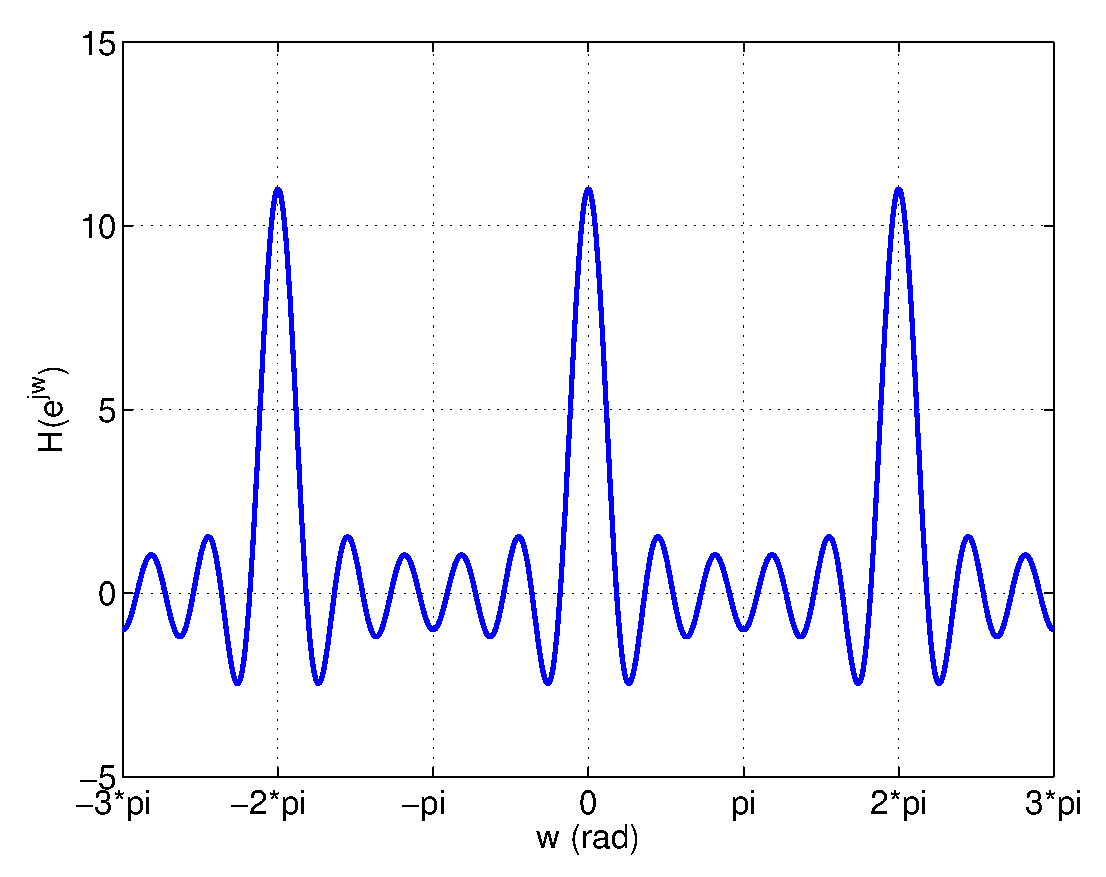
\includegraphics[width=5cm]{./Figures/DFT1.eps}

      \visible<2->{
      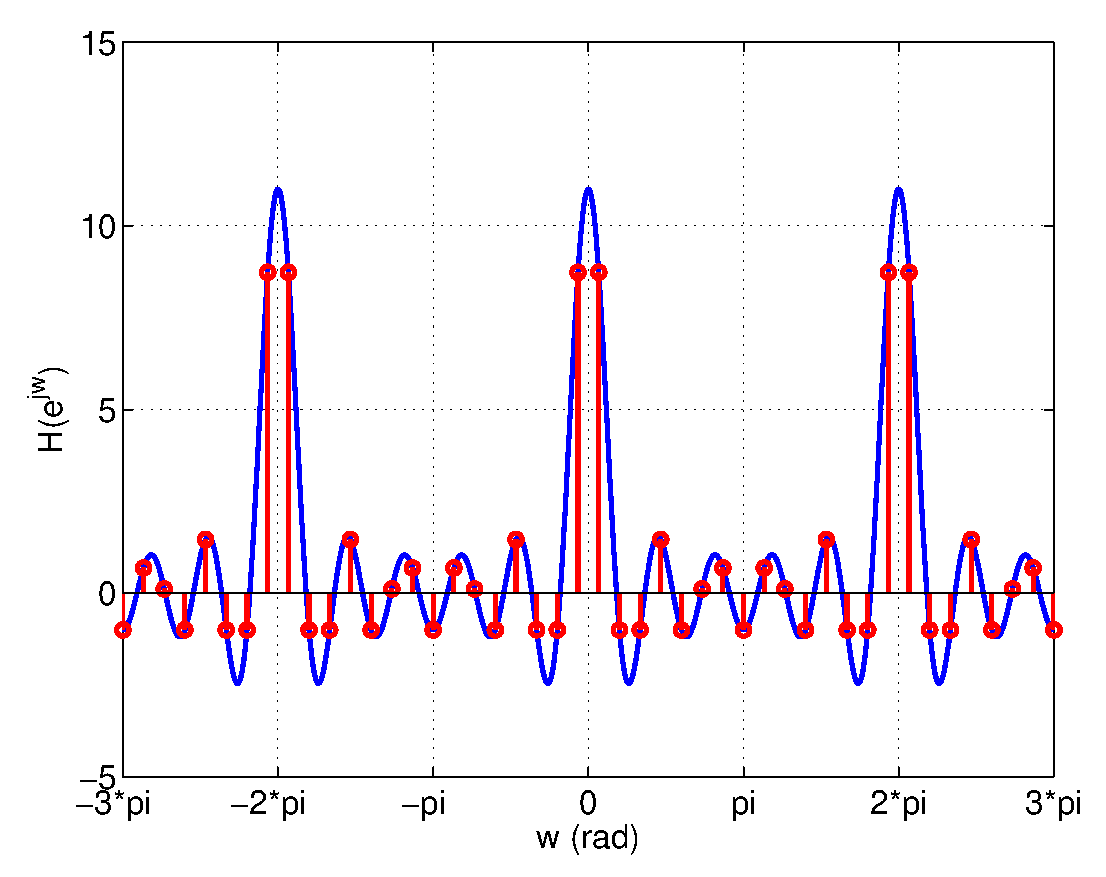
\includegraphics[width=5cm]{./Figures/DFT2.eps}}
    \end{column}
  \end{columns}
\end{frame}

%%%%%%%%%%%%%%%%%%%%%%%%%%%%%%%%%%%%%

\begin{frame}
  \frametitle{Muestreo en el dominio de la frecuencia II}

  \begin{itemize}
    \footnotesize
    \item ¿Como muestreamos de la DTFT ($X(e^{jw})$)?
    \vspace{-0.45cm}
    \begin{columns}[c]
      \hspace{0.9cm}\begin{column}{7cm}
        \begin{itemize}
          \footnotesize
          \visible<2->{\item Para muestrear periódicamente una señal continua $x_a(t)$ en el tiempo, sustituíamos $t=nT$, y hacíamos $x(n)=x_a(nT)$}
          \vspace{-0.1cm}
          \visible<3->{\item Para muestrear la DTFT de la señal discreta, que es continua en $w$, tendremos que hacer $w=k\Delta w$ y $X(k)=X(e^{j\Delta w k})$. }
        \end{itemize}
      \end{column}
      \hspace{-0.8cm}\begin{column}{4cm}
        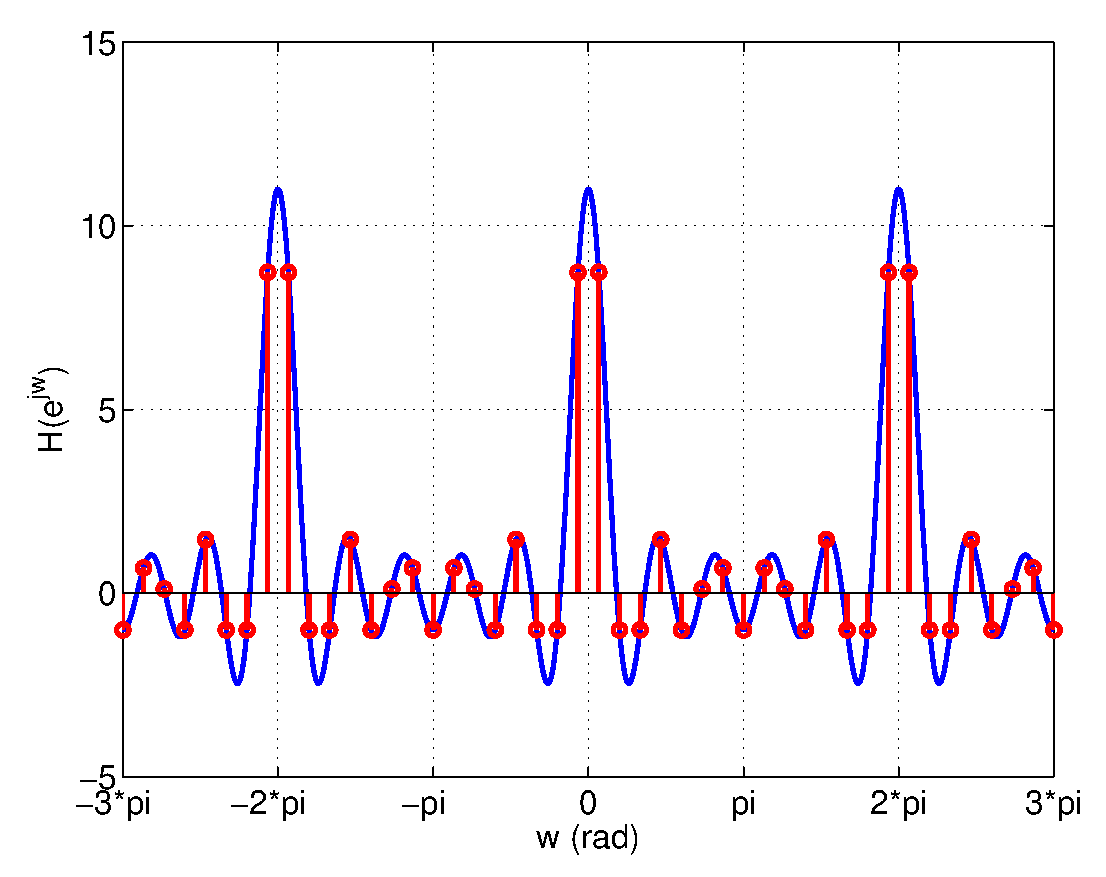
\includegraphics[width=4cm]{./Figures/DFT2.eps}
      \end{column}

    \end{columns}

    \vspace{-0.3cm}

    \begin{itemize}
      \footnotesize
      \visible<4->{\item Para elegir $\Delta w$:}
      \begin{itemize}
        \visible<5->{\item Tenemos en cuenta que $X(e^{jw})$ tiene periodo $2\pi$, y por lo tanto, únicamente es necesario tomar las muestras en el periodo fundamental $[0,2\pi)$}
        \visible<6->{\item Si queremos tomar $N$ muestras equiespaciadas entre $[0,2\pi)$ hacemos de $\Delta w=\frac{2\pi}{N}$}
      \end{itemize}

      \vspace{-0.1cm}

      \visible<7->{
      \item \alert{Las muestras de la DTFT, $X(k)=X(e^{j\frac{2\pi}{N}k})$, reciben el nombre de la Transformada de Fourier Discreta (DFT).} }

      \vspace{0.1cm}

      \visible<8->{
      \scriptsize
      \item La DFT es una señal periódica de periodo N, ya que debido a la periodicidad de la señal $X(e^{jw})$ y el muestreo realizado, cada N muestras la señal se repite. \visible<9->{Ojo: esto no significa que la señal original x(n) tenga que ser periódica. }}
    \end{itemize}

  \end{itemize}
\end{frame}

%%%%%%%%%%%%%%%%%%%%%%%%%%%%%%%%%%%%%%%%%%%%%%%%%%%%%%

\begin{frame}
\frametitle{Reconstrucción de la señal en tiempo discreto I}

  \footnotesize

  \alert{¿Dada la DFT ($N$ muestras de $X(k)$) podemos reconstruir la señal original $x(n)$?}

  \begin{itemize}
    \visible<2->{\item En general no. Pero en algunos casos, si. A continuación analizamos que condiciones se tienen que cumplir, salvo para el caso particular de una señal periódica discreta (relación con la DTFS).}
    \visible<3->{\item Definición de la $X(k)$ a partir de la definición de la $X(e^{jw})$:
    \vspace{-0.1cm}
    $X(e^{jw})=\sum_{n=-\infty}^{\infty} x(n)e^{-jwn}$  $\:\:\: \xrightarrow{w=\frac{2\pi k}{N}}\:\:\: X(k)=\sum_{n=-\infty}^{\infty} x(n)e^{-j\frac{2\pi}{N}kn}$}

    \visible<4->{
    \item Dividimos el sumario sobre n en sumarios de N términos y operamos:

    \scriptsize
    \hspace{-0.7cm}$\alert{X(k)\!=}\!\dots\!+\!\sum_{n=-N}^{-1} x(n)e^{-j\frac{2\pi}{N}\!kn}\!+\!\sum_{n=0}^{N-1} x(n)e^{-j\frac{2\pi}{N}\!kn}\!+\!\sum_{n=N}^{2N-1} x(n)e^{-j\frac{2\pi}{N}\!kn}\!+\!\dots=$}

    \visible<5->{
    $=\!\dots\!+\!\sum_{n=0}^{N-1} \!\!x(n-N)e^{-j\frac{2\pi}{N}\!k(n-N)}\!+\!\sum_{n=0}^{N-1} \!\! x(n)e^{-j\frac{2\pi}{N}\!kn}\!+\!\sum_{n=0}^{N-1} \!\!x(n+N)e^{-j\frac{2\pi}{N}\!k(n+N)}\!+\!\dots$
    }
    \visible<6->{
    $=\!\dots\!+\!\sum_{n=0}^{N-1} \!\!x(n-N)e^{-j\frac{2\pi}{N}\!kn}\!+\!\sum_{n=0}^{N-1} \!\! x(n)e^{-j\frac{2\pi}{N}\!kn}\!+\!\sum_{n=0}^{N-1} \!\!x(n+N)e^{-j\frac{2\pi}{N}\!kn}\!+\!\dots$
    }
    \visible<7->{
    $=\sum_{l=-\infty}^{\infty}\sum_{n=0}^{N-1} x(n-lN) e^{-j\frac{2\pi}{N}\!kn}=\alert{\sum_{n=0}^{N-1}\sum_{l=-\infty}^{\infty} x(n-lN) e^{-j\frac{2\pi}{N}\!kn}}$}

    \visible<8->{
    \footnotesize
    \item Definimos \alert{$x_p(n)=\sum_{l=-\infty}^{\infty} x(n-lN)$}, cuyo valor en un instante $n$ resulta ser el valor que se obtiene sumando los valores de $x(n)$ cada $N$ muestras.}\visible<9->{  Entonces, $\alert{X(k)=\sum_{n=0}^{N-1} x_p(n) e^{-j\frac{2\pi}{N}\!kn}}$.}

    \visible<10->{
    \item Por definición $x_p(n)$ es una función periódica de periodo N:

    $x_p(n+N)=\sum_{l=-\infty}^{\infty} x(n-lN+N) =\sum_{l=-\infty}^{\infty} x(n-lN) =x_p(n)$
    }

  \end{itemize}
\end{frame}

%%%%%%%%%%%%%%%%%%%%%%%%%%%%%%%%%%%%%%%%%%%%%%%%


\begin{frame}
\frametitle{Reconstrucción de la señal en tiempo discreto II}

\vspace{-0.2cm}
\footnotesize
  \begin{itemize}
  \item $\alert{X(k)\!=\!X(e^{j\frac{2\pi}{N}k})\!=\!\sum_{n=0}^{N-1} x_p(n) e^{-j\frac{2\pi}{N}\!kn}}$, transformada de Fourier discreta.
  \item $\alert{x_p(n)\!=\!\sum_{l=-\infty}^{\infty} x(n\!-\!lN)}$, extensión periódica de la señal original.
  \item X(k) y $x_p(n)$ periódicas (periodo N) por construcción.

  \visible<2->{
  \item Como $x_p(n)$ es periódica, podemos representarla a través de su desarrollo en Serie de Fourier (DTFS):}

  \visible<3->{

  \begin{itemize}
  \scriptsize
  \item $x_p(n)=\sum_{k=0}^{N-1} c_k e^{j\frac{2\pi}{N}kn}$}

  \visible<4->{
  \vspace{0.1cm}

  \item $c_k=\frac{1}{N}\sum_{n=0}^{N-1} x_p(n) e^{-j\frac{2\pi}{N}kn}$
  \end{itemize}}
  \visible<5->{
  \item Comparando la expresión de $X(k)$ con la de $c_k$: $c_k=\frac{1}{N}X(k)$.}
  \visible<6->{
  \item Por lo tanto, \alert{$x_p(n)=\frac{1}{N} \sum_{k=0}^{N-1} X(k) e^{j\frac{2\pi}{N}kn}$}.}
  \visible<7->{
  \item La señal periódica $x_p(k)$ se puede reconstruir directamente a partir de la transformada de Fourier discreta ($X(k)$), es decir de las muestras tomadas de la transformada de Fourier en tiempo discreto ($X(e^{jw})$) }
  
  \end{itemize}
  \visible<8->{
  \alert{¿Dada la DFT ($N$ muestras de $X(k)$) podemos reconstruir la señal original $x(n)$?}}
  
  \begin{itemize}
  \visible<9->{
  \item  Si la señal x(n) es de duración finita (distinta de cero sólo durante $L$ instantes sucesivos) y  $L \le  N$, entonces $x_p(n)=x(n)$ y podemos reconstruir la señal original.}
  \item \visible<10->{ Si $L>N$, $x_p(n)\ne x(n)$, se produce aliasing, y la reconstrucción exacta no es posible. }
  \end{itemize}

\end{frame}

%%%%%%%%%%%%%%%%%%%%%%%%%%%%%%%%%%%%


\begin{frame}
\frametitle{Reconstrucción de la señal en tiempo discreto III}

  \footnotesize
  Resumiendo:


  \begin{itemize}
    \item Dada la señal discreta $x(n)$ de duración finita $L$ y su extensión periódica $x_p(n)\!=\!\sum_{l=-\infty}^{\infty} x(n\!-\!lN)$
  \end{itemize}

  \vspace{-0.3cm}
  \vspace{-0.1cm}
  \begin{columns}[c]
    \begin{column}{7.5cm}
      \begin{itemize}
        \item Se tiene que: 

        \begin{itemize}
          \vspace{-0.2cm}
          \footnotesize
          \item ${X(k)\!=\!\sum_{n=0}^{N-1} x_p(n) e^{-j\frac{2\pi}{N}\!kn}}$

          \vspace{0.1cm}

          \item $x_p(n)=\frac{1}{N} \sum_{k=0}^{N-1} X(k) e^{j\frac{2\pi}{N}kn}$
        \end{itemize}
          \visible<2->{
          \item Si $L \le N$:
          \begin{itemize}
          \vspace{-0.4cm}
          \footnotesize
          \item $x_p(n)\!=\!\left\{\!\! \begin{array}{l} x(n), \:\:\:\:\:\:\:\:0\!\le \!n \!\le \!L\!-\!1 \\ 0,  \:\:\:\:\:\:\:\:L\!+\!1\!\le\! n \!\le \!N\!-\!1 \\ x_p(n\!+\!N), \:\:c.c \end{array} \right .$

          \vspace{0.1cm}

          \item $X(k)=\!\sum_{n=0}^{N-1} x(n) e^{-j\frac{2\pi}{N}\!kn}$ 

          \vspace{0.1cm}

          \item $x(n)=\frac{1}{N} \sum_{k=0}^{N-1} X(k) e^{j\frac{2\pi}{N}kn}$

      \end{itemize}}

      \visible<3->{
      \item Si $L>N$ podemos obtener $x_p(n)$ y $X(k)$, pero no $x(n)$, ya que no somos capaces de obtener la $x(n)$ a partir de la $x_p(n)$ o de la $X(k)=X(e^{j\frac{2\pi}{N}k})$.
      }


      \end{itemize}
    \end{column}
    \hspace{-0.9cm}\begin{column}{4cm}
      \visible<1->{
      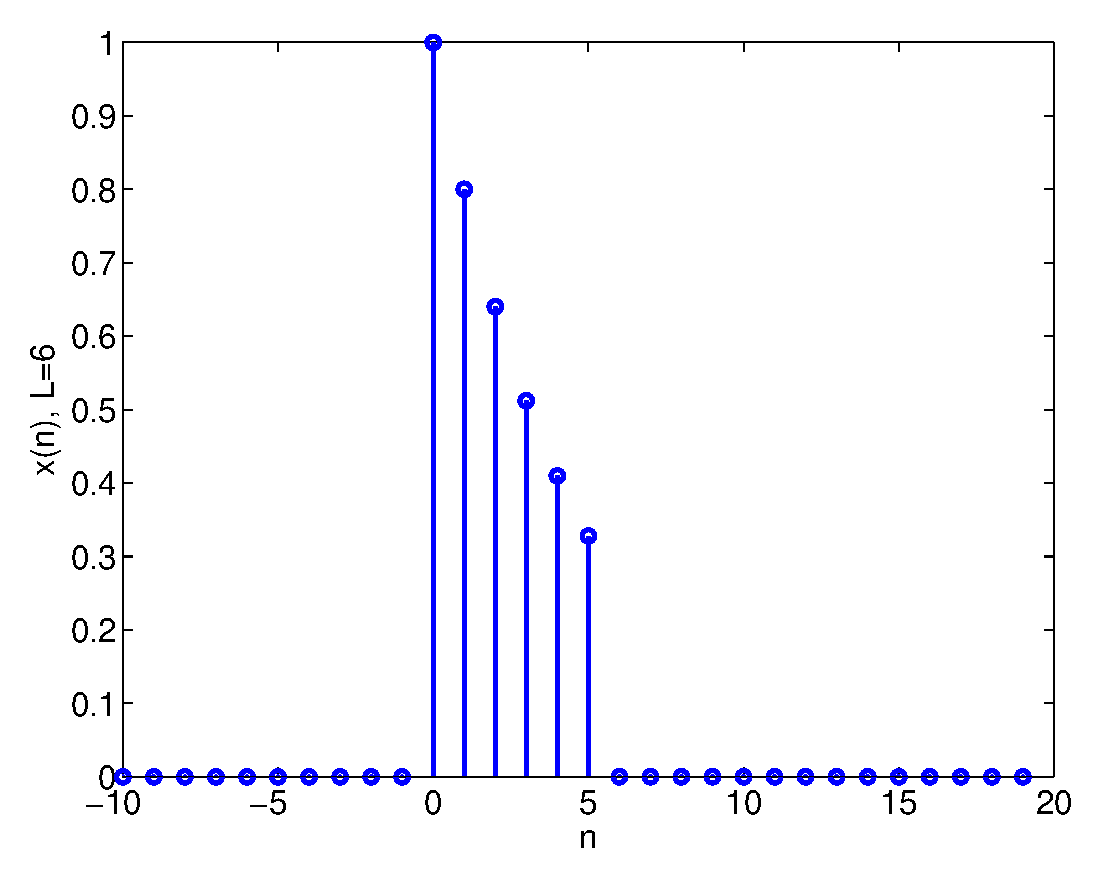
\includegraphics[width=3.5cm,height=2cm]{./Figures/DFTRecXn1.eps}}
      \visible<2->{
      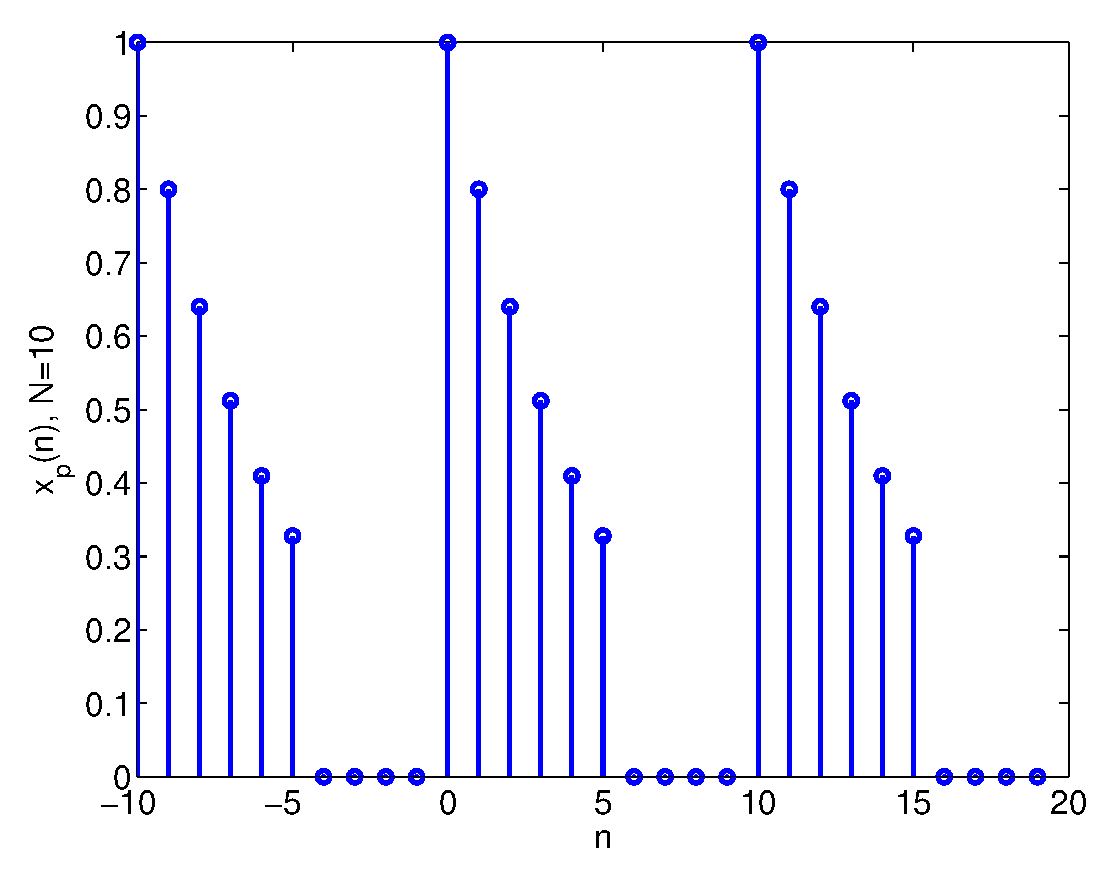
\includegraphics[width=3.5cm,height=2cm]{./Figures/DFTRecXn2.eps}}
      \visible<3->{
      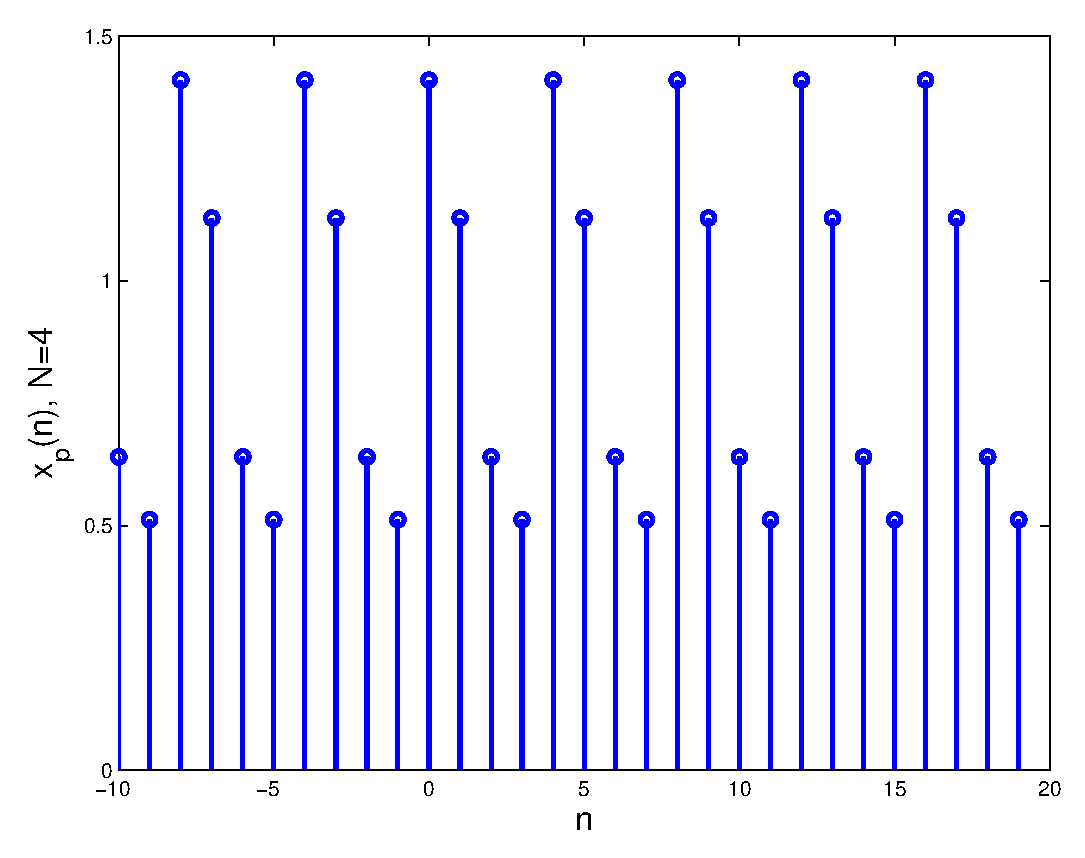
\includegraphics[width=3.5cm,height=2cm]{./Figures/DFTRecXn3.eps}}
    \end{column}
  \end{columns}

\end{frame}

%%%%%%%%%%%%%%%%%%%%%%%%%%%%%%%%%%%%%%%%%%%

\begin{frame}
\frametitle{Reconstrucción de transformada de Fourier I}

  \footnotesize

  \alert{¿Dada la DFT ($N$ muestras de $X(k)$) podemos reconstruir la DTFT ($X(e^{jw})$)?}
 
  \begin{itemize}

    \visible<2->{\item Definición de DTFT: $X(e^{jw})=\sum_{n=-\infty}^{\infty}x(n)e^{-jwn}$}
    \visible<3->{\item Manipulamos la expresión de la DTFT  para buscar la relación entre $X(e^{jw})$ y sus muestras $X(k)$:}
    \begin{itemize}
      \footnotesize
      \visible<4->{\item Como $x(n)$ tiene  longitud finita L, podemos realizar el sumario únicamente sobre los L términos consecutivos de x(n) donde la señal no es cero. Sin embargo, resulta más conveniente hacerlo sobre los N términos, ya que tenemos N muestras en X(k). }
      \visible<5->{
      \item Sustituimos $x(n)=\frac{1}{N} \sum_{k=0}^{N-1} X(k) e^{j\frac{2\pi}{N}kn}$}
      \vspace{0.1cm}
      \visible<6->{\item Reorganizamos sumatorios.}
      \vspace{0.1cm}
      \visible<7->{\item Definimos la función de interpolación $P(e^{jw})=\frac{1}{N}\sum_{n=0}^{N-1}e^{-jwn}$}
    \end{itemize}

    \visible<3->{$\alert{X(e^{jw})}\! =$}\visible<4->{$\sum_{n=0}^{N-1}\!x(n)e^{-jwn}\!=$}\visible<5->{$\sum_{n=0}^{N-1}\!\!\left [\!\frac{1}{N} \sum_{k=0}^{N-1} \!X(k) e^{j\frac{2\pi}{N}kn}\right ] \!\!e^{-jwn}\!=$}
    
    \visible<6->{\hspace{0.9cm} $\!=\!\sum_{k=0}^{N-1} \!X(k) \!\! \left [\frac{1}{N}\sum_{n=0}^{N-1}  e^{j\frac{2\pi}{N}kn} e^{-jwn}\right ]\!=$}

    \visible<6->{\hspace{0.9cm} $\!=\!\sum_{k=0}^{N-1} \!X(k)\! \left [\frac{1}{N}\sum_{n=0}^{N-1}e^{-j(w-\frac{2\pi}{N}k)n}\right ]=$}

    \visible<7->{\hspace{0.9cm}$\alert{=\!\sum_{k=0}^{N-1}\! \!X(k) P(e^{j(w-\frac{2\pi}{N}k)})}$}

  \end{itemize}

\end{frame}

%%%%%%%%%%%%%%%%%%%%%%%%%%%%%%%%%%%%%%%%%%

\begin{frame}
\frametitle{Reconstrucción de transformada de Fourier II}

  \footnotesize

  \alert{¿Dada la DFT ($N$ muestras de $X(k)$) podemos reconstruir la DTFT ($X(e^{jw})$)?}
  
  \footnotesize

  \begin{itemize}
    \item   $X(e^{jw})\! =\!\sum_{k=0}^{N-1}\! \!X(k) P(e^{j(w-\frac{2\pi}{N}k)})$    {\scriptsize \color{gray}(DFT $\leftarrow$ DTFT  para x(n) de longitud finita $L\le N$)\color{black}}
    \item $P(e^{jw})=\frac{1}{N}\sum_{n=0}^{N-1}e^{-jwn}$  {\scriptsize \color{gray}(función de interpolación)\color{black}}

  \end{itemize}

  \begin{columns}[T]
    \begin{column}{6.5cm}
      \begin{itemize}
        \visible<4->{\item Reescribir la expresión de la función de interpolación:}

        \begin{itemize}
          \footnotesize
          \visible<5->{\item $\sum_{n=0}^{N-1} a^n=\frac{1-a^N}{1-a}$}
          \vspace{0.1cm}
          \visible<6->{\item Sacar factor común del numerador y denominador.}
          \vspace{0.1cm}
          \visible<7->{\item Simplificar.}
        \end{itemize}
        \visible<4->{$P(e^{jw})=$}\visible<5->{$\frac{1}{N}\frac {1-e^{-jwN}}{1-e^{-jw}}=$}
        \visible<6->{\hspace{1cm}$=\frac{1}{N}\frac{e^{-j\frac{wN}{2}}}{e^{-j\frac{w}{2}}}\frac {e^{j\frac{wN}{2}}-e^{-j\frac{wN}{2}}}{e^{j\frac{w}{2}}-e^{-j\frac{w}{2}}}= $}
        \visible<7->{\hspace{1cm}$=\frac{sen(\frac{wN}{2})}{N sen(\frac{w}{2}) }e^{-j\frac{w(N-1)}{2}} $}

      \end{itemize}
    \end{column}
    \begin{column}{5cm}
      \visible<2-|handout:1>{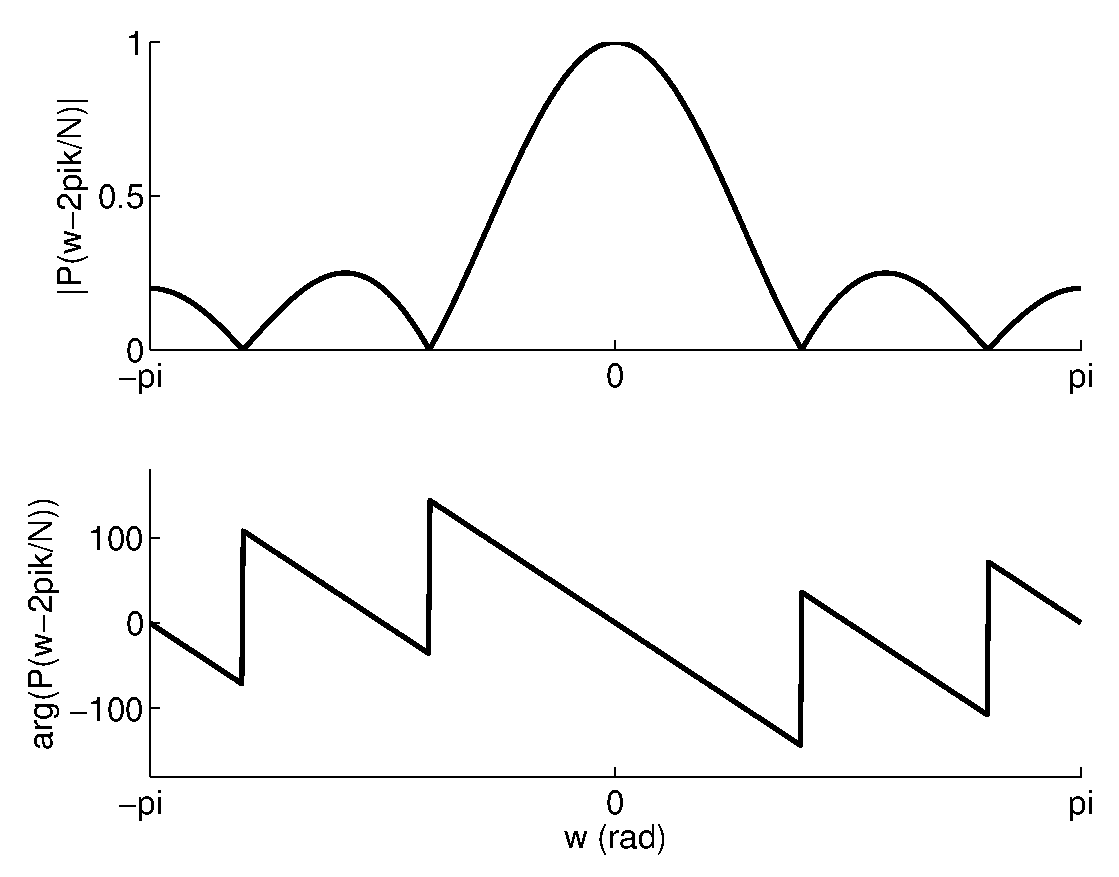
\includegraphics[width=3.5cm]{./Figures/DFTRecHw1.eps}}
      \visible<3-|handout:1>{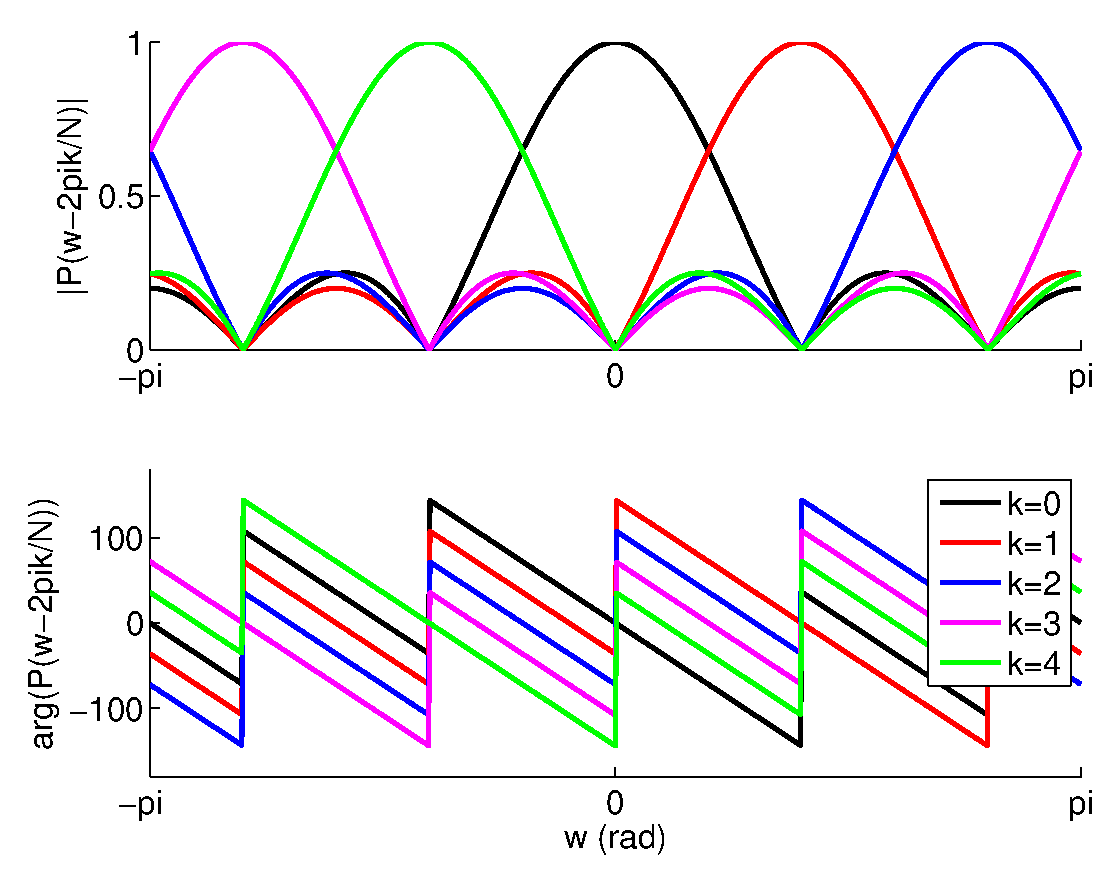
\includegraphics[width=3.5cm]{./Figures/DFTRecHwN.eps}}
    \end{column}
  \end{columns}

\end{frame}

% \begin{frame}
  \frametitle{Definición de la transformada de Fourier Discreta}

  \footnotesize
  \begin{itemize}
    \item Una señal discreta $x(n)$ de longitud finita L  (x(n)=0 $n\ge L$)
    \item Transformada de Fourier Discreta (DFT) de N muestras ($N \ge L$):
    \hspace{0.5cm} \alert{$X(k)=X(e^{j\frac{2\pi}{N}k})=\sum_{n=0}^{N-1} x(n) e^{-j\frac{2\pi}{N}kn}$}   para $k=\{0,\dots,N-1\}$
    \item Transformada de Fourier Discreta Inversa (IDFT):
    \hspace{0.5cm} \alert{$x(n)=\frac{1}{N}\sum_{k=0}^{N-1} X(k) e^{j\frac{2\pi}{N}kn}$}

    \item Observaciones:
    \begin{itemize}
    \footnotesize
      \item Si $L < N$ la expresión de la IDFT da x(n)=0 para $n\ge L$.
      \item La DFT de una señal de duración infinita siempre se obtendrá con aliasing
      \item Para cualquier señal $x(n)$ de duración finita de longitud L, cualquier DFT con $N\ge L$ obtenida a partir de la extensión periódica $x_p(n)$ de la señal original, permite obtener unívocamente su DTFT $X(e^{jw})$ utilizando la función de interpolación $P(e^{jw})$.
      \item Una mayor diferencia entre N y L no suministra mayor información sobre el espectro $X(e^{jw})$, aunque permite representarlo en más puntos (los N de la DFT).
    \end{itemize}
  \end{itemize}
\end{frame}
% 

%%%%%%%%%%%%%%Empieza la presentacion%%%%%%%%%%%%%%%%%%%%%%%%%%%%%%%%%%%%

%\begin{frame}
%\frametitle{Esquema}
 %   \tableofcontents
%\end{frame}

\section{Relación de la DTF con otras transformadas}


%%%%%%%%%%%%%%%%%%%%%%%%%%%%%%

\begin{frame}
\frametitle{Relación con la Serie de Fourier Discreta}


\vspace{-0.2cm}

\footnotesize
\begin{itemize}
 \item \alert{Relación entre las señales periódicas discretas y la DFT:}

\hspace{0.5cm}\alert{¿Dada una señal periódica discreta cual es su DFT ?}

\hspace{0.5cm}\alert{¿Relación existe entre los coeficientes de la DTFS y la DFT ?}
\end{itemize}

\vspace{-0.3cm}

\visible<2->{

\begin{columns}[T]
\hspace{0.4cm}\begin{column}{6cm}
\begin{itemize}
\item Señal periódica discreta:

$x(n+N)=x(n)$

$x(n)=\sum_{k=0}^{N-1}c_ke^{j\frac{2\pi}{N}kn}$

$c_k=\frac{1}{N}\sum_{n=0}^{N-1}x(n)e^{-j\frac{2\pi}{N}kn}$

\end{itemize}
\end{column}


\begin{column}{6cm}
\begin{itemize}
\item DFT:

$x(n)$ de longitud finita $L \le N$

$x(n)=\frac{1}{N}\sum_{k=0}^{N-1} X(k) e^{j\frac{2\pi}{N}kn}$

$X(k)=\sum_{n=0}^{N-1} x(n) e^{-j\frac{2\pi}{N}kn}$

\end{itemize}
\end{column}
\end{columns}

}

\begin{itemize}
\visible<3->{\item Comparando las expresiones:  \alert{$c_k=X(k)/N$}.}
\visible<4->{\item La serie de Fourier tiene la estructura de la DFT.  Si definimos la secuencia de duración finita como los N puntos de la señal periódica se tiene $X(k)=Nc_k$.}
\visible<5->{\item La expresión de síntesis de la serie tiene la estructura de la IDFT. Por lo tanto, los $N$ puntos de la DFT nos proporcionan las lineas del espectro de la secuencia periódica de periodo fundamental N.}
\visible<6->{\item Finalmente, como $X(k)=X(e^{j\frac{2\pi k}{N}})$, y la señal periódica tiene una DTFT que es un tren de pulsos sobre las frecuencia fundamental, es necesario muestrear la DFT con el mismo periodo que el de la señal discreta original para evitar que se pierda algún armónico en la X(k).}

\end{itemize}

\end{frame}


%%%%%%%%%%%%%%%%%%%%%%%%%%%%%%

\begin{frame}
\frametitle{Relación con la DTFT}

\footnotesize

\alert{Relación entre la DFT y la DTFT:}

\begin{itemize}
\footnotesize
\item Hemos visto la relación en la introducción. Resumimos:
\item $x(n)$ es una secuencia aperiódica con DTFT $X(e^{jw})$ los N valores de la DFT son $X(k)=X(e^{j\frac{2\pi k}{N}})$.

\item Los X(k) son los coeficientes de la señal periódica $x_p(n)=\sum_{l=-\infty}^{\infty} x(n-lN)$.

\item Si la secuencia x(n) es de duración finita$^{1}$ $L\le N$, entonces los X(k) permiten recuperar la secuencia x(n) a través de la IDFT.

\item Si la secuencia no tiene duración finita o su duración es $L>N$ la IDFT no permite recomponer la señal, ya que aunque sus N coeficientes permitirán obtener la señal periódica $x_p(n)=\sum_{l=-\infty}^{\infty} x(n-lN)$, no podríamos extraer de los mismos los valores de la señal original.

\item Si la secuencia x(n) es de duración finita$^{1}$ $L\le N$, $X(e^{jw})=\!\sum_{k=0}^{N-1} \!X(k)\! \left [\frac{1}{N}\sum_{n=0}^{N-1}e^{-j(w-\frac{2\pi}{N}k)n}\right ]= \!\sum_{k=0}^{N-1} \!X(k)\! \frac{sen(\frac{w_kN}{2})}{N sen(\frac{w_k}{2}) }e^{-j\frac{w_k(N-1)}{2}}$ con $w_k=w-\frac{2\pi}{N}k$

\vspace{-0.2cm}

\rule{11cm}{0.4pt}

 $^1$Las señales periódicas son un caso excepcional a esta norma siempre y cuando el periodo de la señal y el número de muestras de la DFT coincidan.

\end{itemize}


\end{frame}

%%%%%%%%%%%%%%%%%%%%%%%%%%%%%%

\begin{frame}
\frametitle{Relación con la Transformada Z}

\footnotesize

\alert{¿Podemos obtener los N términos $X(k)$ de la DFT a partir de la Transformada Z?}

\begin{itemize}
\visible<2->{\item $X(k)=X(e^{j\frac{2\pi k}{N}})$}
\visible<3->{\item $X(e^{jw})=X(z)|_{z=e^{jw}}$}
\visible<4->{\item Por lo tanto la DFT se puede obtener muestreando de la Transformada Z sobre N puntos equiespaciados del círculo unidad.}
\end{itemize}


\alert{¿Podemos obtener la Transformada Z a partir de los N términos $X(k)$ de la DFT?}

\begin{itemize}

\visible<5->{\item Definición de la Transformada Z: $X(z)=\sum_{n=-\infty}^{\infty} x(n) z^{-n}$}

\visible<6->{\item Si la x(n) es de longitud finita $\le N$:

$X(z)=\sum_{n=0}^{N-1} x(n) z^{-n}=\sum_{n=0}^{N-1}\left [\frac{1}{N}\sum_{k=0}^{N-1} X(k)e^{j \frac{2\pi k n}{N}} \right ] z^{-n}=$

\hspace{1cm}$=\frac{1}{N} \sum_{k=0}^{N-1} X(k) \sum_{n=0}^{N-1} \left [e^{j \frac{2\pi k}{N}} z^{-1}\right ]^n=
\frac{1}{N} \sum_{k=0}^{N-1} X(k)  \frac{ 1- e^{j \frac{2\pi Nk}{N}} z^{-N}}{1-e^{j \frac{2\pi k}{N}} z^{-1}} =$

\hspace{1cm}$=\frac{1-z^{-N}}{N} \sum_{k=0}^{N-1} \frac{ X(k)  }{1-e^{j \frac{2\pi k}{N}} z^{-1}}$

 }

\end{itemize}

\end{frame}

%%%%%%%%%%%%%%%%%%%%%%%%%%%%%%

\begin{frame}
\frametitle{Relación con la Serie de Fourier Continua}

\footnotesize

\hspace{1cm}\alert{¿Relación existe entre los coeficientes de la CTFS y la DFT ?}

\visible<2->{

\begin{itemize}
\item Establecemos la relación a través de la IDFT y la CTFS.
\item IDFT de una señal discreta: $x(n)=\frac{1}{N}\sum_{k=0}^{N-1}X(k)e^{j\frac{2\pi}N kn}$
\item Señal  continua $x_a(t)$  periódica con periodo $T$
\item $x_a(t)$  periódica $\rightarrow$ definida con su serie de Fourier: $x_a(t)=\sum_{k=-\infty}^\infty c_k e^{j\frac{2\pi}{T}kt}$
\item  Muestreando $x_a(t)$ con periodo de muestreo $T_s=\frac{T}{N}$ tenemos la señal discreta $x(n)=x_a(T_sn)=x_a(\frac{Tn}{N})$.

$x(n)=x_a(T_sn)= \sum_{k=-\infty}^\infty c_k e^{j\frac{2\pi}{T}k \frac{Tn}{N}}=\sum_{k=-\infty}^\infty c_k e^{j\frac{2\pi }{N}kn}$

\hspace{0.7cm}$=\sum_{k=0}^{N-1} \left [ \sum_{l=-\infty}^\infty c_{k-lN}  \right ]e^{j\frac{2\pi }{N}kn} $

\vspace{0.1cm}
}
\visible<3->{
\item Relación: $X(k)= N \sum_{l=-\infty}^\infty c_{k-lN}$

\vspace{-0.1cm}

\begin{itemize}
\scriptsize
\item  $\sum_{l=-\infty}^\infty c_{k-lN}$ expansión periódica de los coeficientes de Fourier de la señal continua
\item Si el número de coeficientes no nulos es finito y menor que N, $\sum_{l=-\infty}^\infty c_{k-lN}=c_k$, podemos extraer los coeficientes a partir de la DFT.
\item  Si el número de coeficientes distintos de cero es mayor que N, no podemos obtenerlos a partir de la DFT. De hecho, en general, salvo que nos aseguren que se cumple el caso contrario, este es el que debemos asumir que se cumple, y que por lo tanto, no se pueden recuperar los $c_k$ a partir de la DFT.
\end{itemize}


}

\end{itemize}



\end{frame}

  

%%%%%%%%%%%%%%Empieza la presentacion%%%%%%%%%%%%%%%%%%%%%%%%%%%%%%%%%%%%

%\begin{frame}
%\frametitle{Esquema}
 %   \tableofcontents
%\end{frame}

\section{Propiedades de la DFT}

\begin{frame}\frametitle{Propiedades}
	\begin{itemize}
		\item \alert{Periodicidad}:\\
		\vspace{0.5cm}
		$x[n]\leftrightarrow X[k] \color{blue}\Rightarrow \left\{\begin{aligned}&x[n]=x[n+N]\\&X[k+N]=X[k]\end{aligned}\right.\color{black}$ 

		\vspace{2cm}
		\item \alert{Linealidad}:\\
		\vspace{0.5cm}
		$\begin{aligned}
			&x_1[n]\leftrightarrow X_1[k] \\
			&x_2[n]\leftrightarrow X_2[k] 
		\end{aligned}\color{blue}\Rightarrow
		\alpha_1 x_1[n] + \alpha_2 x_2[n]\leftrightarrow \alpha_1 X_1[k] + \alpha_2 X_2[k]$ \color{black}
	\end{itemize}
\end{frame}

\begin{frame}\frametitle{Propiedades}
	\begin{itemize}
		\item Recordamos:
		\begin{itemize}
			\item Secuencia finita de duración L: \color{blue}$x[n]$\color{black}
			\item Expansión periódica de N puntos: \color{blue}$x_p[n]=\sum_{l=-\infty}^{\infty} x[n-lN]$\color{black}
			\item DFT ($L<N$) es equivalente: \color{blue}$x[n]\leftrightarrow X[n]$\color{black}
		\end{itemize}
		\item \alert{Simetría circular}:
	\end{itemize}

\end{frame}



	% \begin{frame}
% \frametitle{Desplazamiento circular I}

% \footnotesize

% \begin{columns}[T]
% \hspace{-0.5cm}\begin{column}{7cm}
% \begin{itemize}
% \item Señal discreta $x(n)$ $\rightarrow$ Expansión periódica (periodo N) es $x_p(n)\!=\!\sum_{l=-\infty}^{\infty}\!\!x(n\!-\!lN)$
% \visible<2->{\item Si la secuencia tiene longitud finita $L<=N$:}
% \begin{itemize}
% \footnotesize
% \visible<3->{\item Su extensión periódica consiste en repetir la señal periódicamente cada N instantes.}
% \visible<4->{\item El desplazamiento $x_p(n)$ en el dominio temporal de k unidades  $x_p(n-k)$}\visible<5->{ induce un desplazamiento circular la señal original. }

% \item \visible<6->{La señal circular desplazada se representa como $x((n-k)_N)$}.

% \scriptsize{


%  \visible<7->{
% \vspace{0.2cm}

% \hspace{-0.4cm}\color{olivegreen}{Ejemplo: $y(n)=x((n-k)_N)$ con  $N=5, k=2$}}

% \vspace{0.1cm}

%  \visible<8->{
% \color{gray}
% $y(0)=x((0-2)_5)=x(-2+5)=x(3)$
% $y(1)=x((1-2)_5)=x(-1+5)=x(4)$
% $y(2)=x((2-2)_5)=x(0)$
% $y(3)=x((3-2)_5)=x(1)$
% $y(4)=x((4-2)_5)=x(2)$}}


% \end{itemize}
% \end{itemize}
% \end{column}
% \hspace{-0.3cm}\begin{column}{4cm}
% \only<2|handout:0>{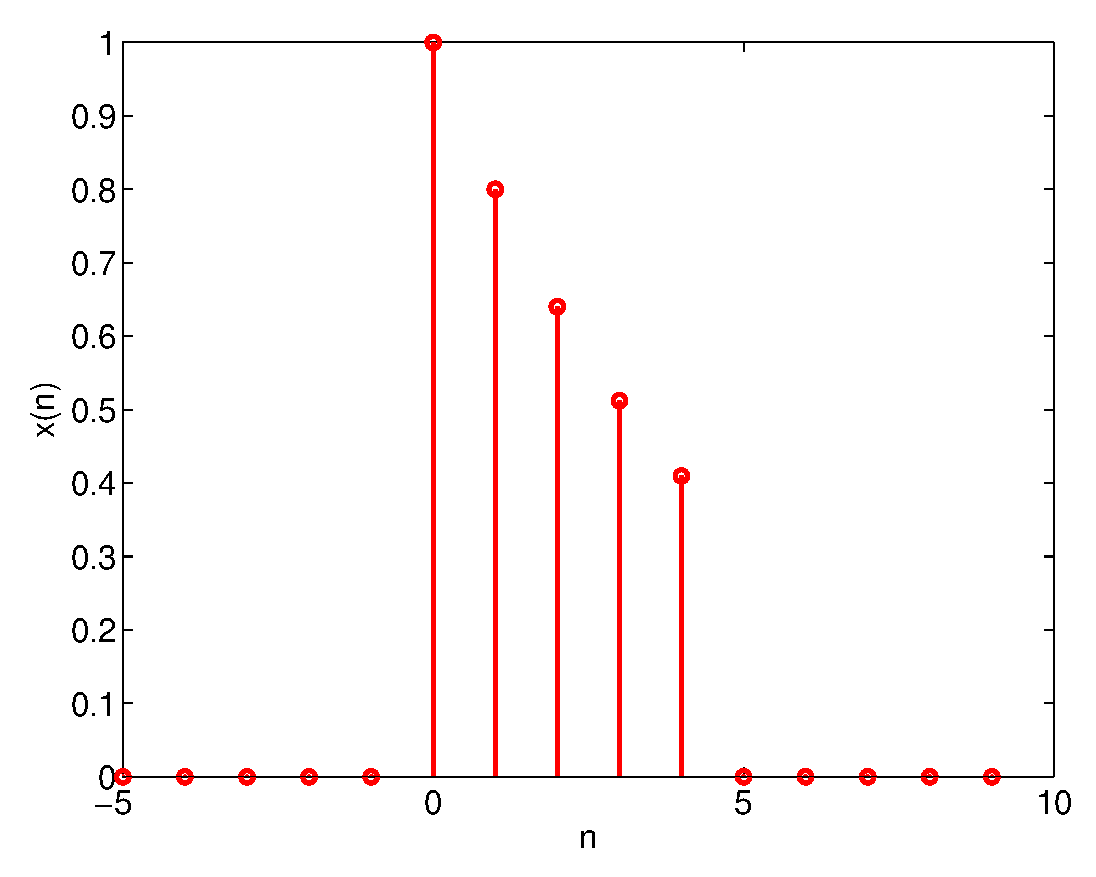
\includegraphics[width=4.5cm]{./Figures/Circular1.eps}}\visible<3->{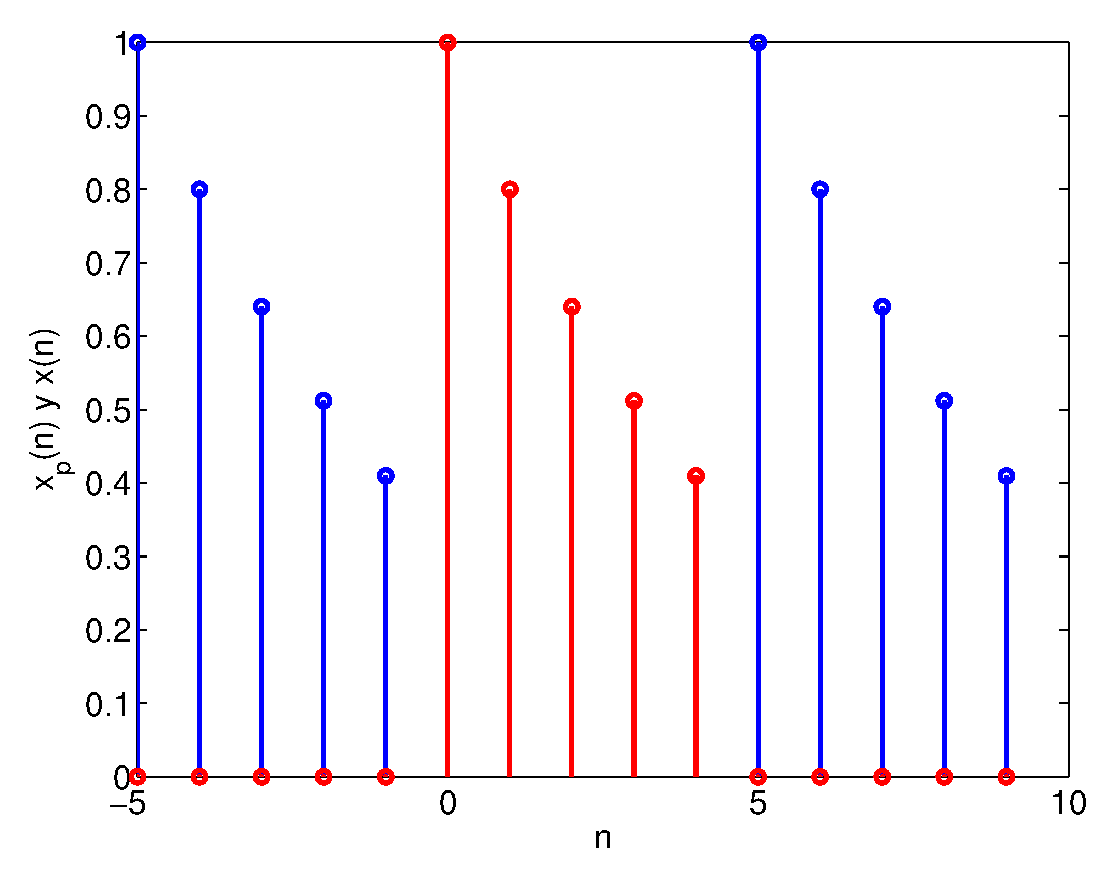
\includegraphics[width=4.5cm]{./Figures/Circular2.eps}}

% \only<4|handout:0>{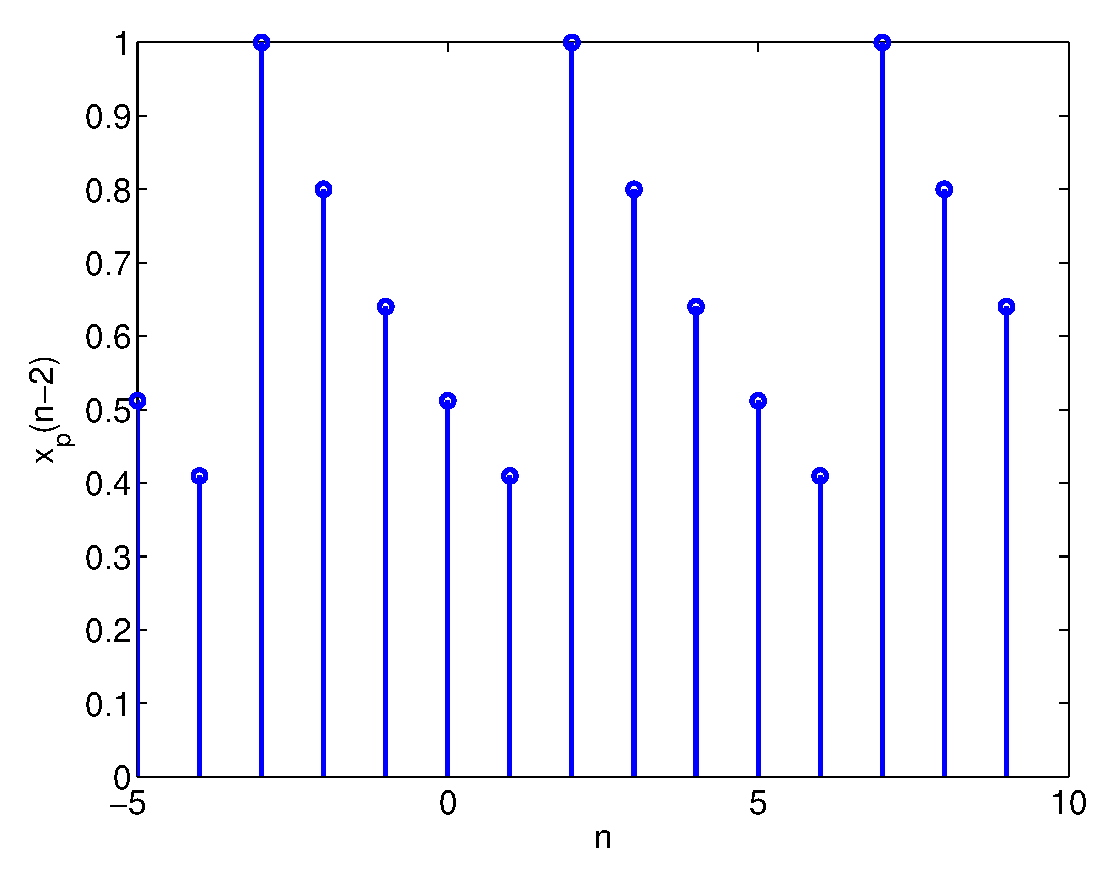
\includegraphics[width=4.5cm]{./Figures/Circular3.eps}}\visible<5->{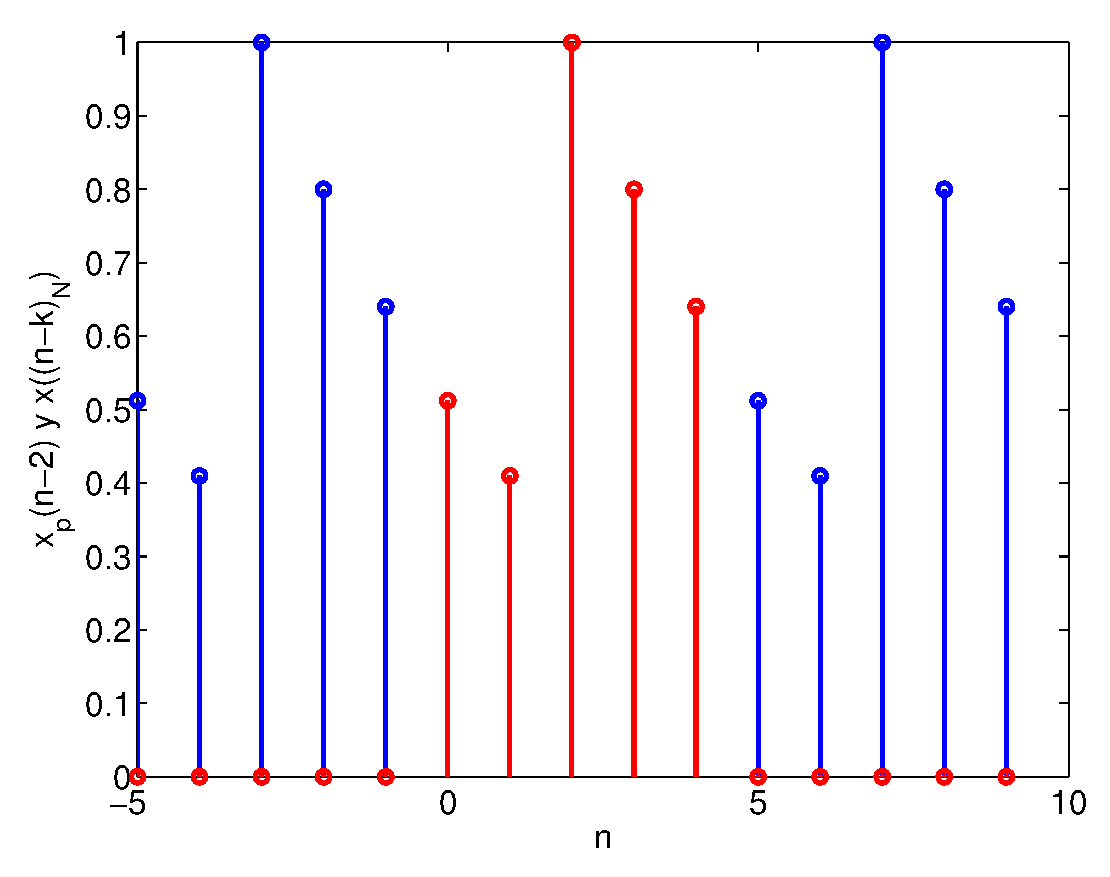
\includegraphics[width=4.5cm]{./Figures/Circular4.eps}}
% \end{column}
% \end{columns}
% \end{frame}

% %%%%%%%%%%%%%%%%%%%%%%%%%%%%%%

% \begin{frame}
% \frametitle{Desplazamiento circular II}

% \footnotesize

% \begin{itemize}
% \item Reflexión temporal: $x((-n)_N)=x(N-n)$
% \item Secuencia circularmente par: $x((-n)_N)=x(n)$  
% \item Secuencia circularmente impar: $x((-n)_N)=-x(n)$   


% \item Propiedades de simetria de la DFT:

% \hspace{2cm}\alert{$X(k)=\sum_{n=0}^{N-1} x(n) e^{-j\frac{2\pi}{N}kn}$}

% \hspace{2cm}\alert{$x(n)=\frac{1}{N}\sum_{k=0}^{N-1} X(k) e^{j\frac{2\pi}{N}kn}$}


% \vspace{0.1cm}

% \hspace{2cm}$x(n)=Re[x(n)]+j \: Im[x(n)]=x_p(n)+x_i(n)$

% \vspace{0.1cm}

% \hspace{5.3cm}$X(k)=X_p(k)+X_i(k)$

% \vspace{0.1cm}

% \begin{tabular}{|c|c|}

% \hline
% Secuencia & DFT \\ \hline
% $x(n)$ & $X(k)$ \\ \hline
% \alert{$x^*(n)$} & \alert{$X^*(N-k)$} \\ \hline
% \alert{$x^*(N-n)$} & \alert{$X^*(k)$} \\ \hline
% $Re[x(n)]=\frac{x(n)+x^*(n)}{2}$ & $\frac{X(k)+X^*(N-k)}{2}=\frac{X_p(k)+X_i(k)+X_p(N-k)-X_i(N-k)}{2}=X_p(k)$ \\ \hline
% $Im[x(n)]=\frac{x(n)-x^*(n)}{2j}$ & $\frac{X(k)-X^*(N-k)}{2j}=\frac{X_p(k)+X_i(k)-X_p(N-k)+X_i(N-k)}{2j}=X_i(k)$ \\ \hline

% $x_p(n)=\frac{x(n)+x(N-n)}{2}$ & $\frac{X(k)+X(N-k)}{2}=\frac{X(k)+X^*(k)}{2}=Re[X(k)]$ \\ \hline
% $x_i(n)=\frac{x(n)-x(N-n)}{2}$ & $\frac{X(k)-X(N-k)}{2}=\frac{X(k)-X^*(k)}{2}=j \: Im[X(k)]$ \\ \hline

% \end{tabular}


% \end{itemize}

% \end{frame}


% %%%%%%%%%%%%%%%%%%%%%%%%%%%%%%%%

% \begin{frame}
% \frametitle{DFT de señales reales}


% \begin{itemize}
% \item Se pueden obtener:
% \begin{itemize}

% \item Utilizando la relación de Euler (tal y como hicimos en el caso de la CTFT y DTFT)
% \item Aprovechando la relación entre la DTFT y la DFT, teniendo en cuenta las diferencias de paridad/imparidad habitual y la circular. 
% \end{itemize}
% \item Propiedades DFT señales reales$^1$:
% \begin{itemize}

% 	\item $x(n) \:\:\: \leftrightarrow \:\:\:X(k)=X^*(N-k)$
% 	\item La componente real de X(k) es par y la imaginaria es impar.
% 	\item Si x(n) es par, X(k) es real y par.
% 	\item Si x(n) es impar, X(k) es imaginaria e impar.
% 	\item El módulo de X(k) es par y el argumento es impar.
% 	\item Si x(n) es par, modulo par, argumento es 0 o $\pi$
% 	\item Si x(n) es impar, modulo impar, argumento $\pi/2$ o $3\pi/2$.
% \end{itemize}


% \end{itemize}

% \rule{11cm}{0.4pt}

% \footnotesize
% $^1$ Con paridad/imparidad circular.

% \end{frame}


% %%%%%%%%%%%%%%%%%%%%%%%%%%%%%%


% \begin{frame}
% \frametitle{Propiedades de la DFT}

% \small
% \hspace{3cm}\alert{\footnotesize $X(k)= \sum_{n=0}^{N-1} x(n) e^{-j\frac{2\pi}{N}kn} $}

% \vspace{0.1cm} 
 
% \hspace{3cm} \alert{\footnotesize  $x(n)=\frac{1}{N} \sum_{n=0}^{N-1} X(k)  e^{j\frac{2\pi}{N}kn}$}

% \vspace{0.2cm}

% Propiedades:

% \vspace{-0.2cm} 

% \begin{itemize}
% \footnotesize
% \item Linealidad: $\:\:\:\:\:\:\:\:\:\:\:\:\:\:\:\:\:\:\:\:\:\:\:\: \:\:\:\:\:\:\:\:\:\:\:\: \:\:\: \:\:\:\alpha x_1(n)+\beta x_2(n) \:\:\:\: \leftrightarrow  \:\:\:\:\alpha X_1(k)+ \beta X_2(k)$
% \item Periodicidad en k: $\:\:\:\:\:\:\:\:\:\:\:\:\:\:\:\:\:\:\:\:\:\:\:\:\:\:\:x(n+N)=x(n)$

% \hspace{2cm}$\:\: \:\:\:\:\:\:\:\: \:\:\:\:\:\:\:\: \:\:\:\:\:\:\:\: \:\:\:\:\:\:\:\: X(k)=X(k+N)$

% \item Desplazamiento temporal circular: $x((n-l)_N)  \:\:\:\:\:\:\:\: \leftrightarrow   \:\:\:\:\:\:\:\: e^{j\frac{-2\pi}{N}kl}X(k)$
% \item Modulación:   $\:\: \:\:\:\:\:\:\:\:\:\:\:\:\:\:\:\:  \:\:\:\:\:\:\:\: \:\:\:\:\:\:\:\:\:\:\:\:\:\:\:\: x(n)e^{j\frac{2\pi}{N}ln}\:\: \:\:\:\:\:\:\:\:  \leftrightarrow \:\:\:\:\:\:\:\: X((k-l)_{N}) $
% \item Convolución circular: $\:\:\:\:\:\:\:\:\:\:\:\:\:\:\:\:\:\:\:\:\:\:\:\:\: (x*y)_{N}(n) \:\:\:\:\:\:\:  \leftrightarrow \:\:\:\:\:\:\:\:   X(k)Y(k)$
% \item Producto circular: $\:\:\:\:\:\:\:\:\:\:\:\:\:\:\:\:\:\:\:\:\:\:\:\:\:\:\:\:\:\:\: x(n)y(n)   \:\:\: \:\:\:\:\:\:\:\:  \leftrightarrow \:\:\:\:\:\:\:\:  \frac{1}{N}(X*Y)_{N}(k)$

% \item $x^*(n) \:\:\:\:\:\:\:\:\:\:\:\:\:\:\:\leftrightarrow \:\:\:\:\:\:\:\:X^*(N-k)$

% \item  $x(N-n)  \:\:\:\:\:\:\:\:    \leftrightarrow   \:\:\:\:\:\:\:\:  X(N-k)$

% \end{itemize}
% \end{frame}
% %%%%%%%%%%%%%%%%%%%%%%%%%%%%%%%%%%%%%%%%%%%%%%


% \begin{frame}
% \frametitle{Convolución circular}

% \footnotesize
% \begin{itemize}
% \item Tenemos dos secuencias finitas de longitud $N$, $x_1(n)$ y $x_2(n)$.
% \item Sus DFTs correspondientes son:

% \hspace{1cm}$X_1(k)=\sum_{n=0}^{N-1}x_1(n)e^{-j \frac{2\pi}{N}kn}$

% \hspace{1cm}$X_2(k)=\sum_{n=0}^{N-1}x_2(n)e^{-j \frac{2\pi}{N}kn}$

% \item Definimos producto de ambas señales en el dominio de la transformada $X_3(k)=X_1(k)X_2(k)$.

% \item Calculamos la IDFT:
% $x_3(m)=\frac{1}{N}\sum_{k=0}^{N-1} X_3(k)e^{j \frac{2\pi}{N}km}=\frac{1}{N}\sum_{k=0}^{N-1} X_1(k)X_2(k)e^{j \frac{2\pi}{N}km}=$
% $=\frac{1}{N}\sum_{k=0}^{N-1} \left[\sum_{n=0}^{N-1}x_1(n)e^{-j \frac{2\pi}{N}kn} \right] \left[\sum_{l=0}^{N-1}x_2(l)e^{-j \frac{2\pi}{N}kl} \right]e^{j \frac{2\pi}{N}km}=$
% $=\frac{1}{N}\sum_{n=0}^{N-1} x_1(n)  \sum_{l=0}^{N-1}x_2(l) \left[ \sum_{k=0}^{N-1}e^{j \frac{2\pi}{N}k(m-n-l)} \right ]=$
% $=\frac{1}{N}\sum_{n=0}^{N-1} x_1(n) N x_2(m-n-pN)=\sum_{n=0}^{N-1} x_1(n) x_2((m-n)|_N)=(x*y)_N(m)$

% \item \alert{$(x*y)_N(m)=\sum_{n=0}^{N-1} x_1(n) x_2((m-n)|_N)  \:\:\:\:   \leftrightarrow \:\:\:\: X(k)Y(k)$}

% \rule{11cm}{0.4pt}

% $\sum_{k=0}^{N-1}e^{j \frac{2\pi}{N}k(m-n-l)} = \left \{\begin{array}{l} N,   \:\:\: m-n-l=pN, p\in \mathcal{Z} \\ 0,  \:\:\: c.c. \end{array}\right .$


% \end{itemize}


% \end{frame}


% \begin{frame}
% \frametitle{Relación entre Convoluciones y T. Fourier }

% \footnotesize
% \begin{itemize}

% \item Definiciones de convolución
% \begin{itemize}

% \footnotesize

% \visible<2->{

% \item Convolución continua: $(x*y)(t)=\int_{-\infty}^{\infty} x(\tau)y(t-\tau)d\tau$
% \item Convolución periódica continua  $(x*y)_T(t)=\int_T x(\tau)y(t-\tau)d\tau$
% \item Convolución discreta: $(x*y)(m)=\sum_{n-\infty}^{\infty} x(n)y(m-n)$
% \item Convolución circular discreta $(x*y)_N(m)=\sum_{n=0}^{N-1} x(n)y((m-n)|_N)$
% }
% \end{itemize}

% \item Transformadas de Fourier:


% \begin{itemize}
% \footnotesize
% \visible<3->{
% \item CTFT:	
% \begin{itemize}
% 	\item Señales genéricas continuas en tiempo y frecuencia.
% 	\item$\mathcal{F}[(x*y)(t)]=X(jw)Y(jw)$       
% 	\item $\mathcal{F}[(x(t)y(t))]=\frac{1}{2\pi}(X*Y)(jw)$
% \end{itemize}}

% \visible<4->{\item DTFT:	
% \begin{itemize}
% 	\item Señal genérica discreta en tiempo y periódica continua en frecuencia.
% 	\item$\mathcal{F}[(x*y)(n)]=X(e^{jw})Y(e^{jw})$       
% 	\item $\mathcal{F}[(x(n)y(n))]=\frac{1}{2\pi}(X*Y)_{2\pi}(e^{jw})$
% \end{itemize}}

% \visible<5->{\item DFT:	
% \begin{itemize}
% 	\item Señal periódica (circular) discreta en tiempo frecuencia.
% 	\item$\mathcal{F}[(x*y)|_N(n)]=X(k)Y(k)$       
% 	\item $\mathcal{F}[(x(n)y(n))]=\frac{1}{N}(X*Y)_{N}(k)$
% \end{itemize}}

% \end{itemize}	


% \end{itemize}


% \end{frame}


%   

%%%%%%%%%%%%%%Empieza la presentacion%%%%%%%%%%%%%%%%%%%%%%%%%%%%%%%%%%%%

%\begin{frame}
%\frametitle{Esquema}
 %   \tableofcontents
%\end{frame}

\section{Sistemas LTI y Filtros Discretos}


%%%%%%%%%%%%%%%%%%%%%%%%%%%%%%

\begin{frame}
\frametitle{Sistemas LTI y Filtros Discretos I}

\footnotesize

\begin{itemize}
\item La respuesta y(n) de un sistema LTI discreto a una entrada  x(n) se calcula:
\begin{itemize}
\footnotesize
\item Como la convolución entre  $x(n)$ y la respuesta del sistema a la entrada impulso $h(n)$:
	$\alert{y(n)}\!=\!T[x(n)]\!=\!(h*x)(n)\!\alert{=\!\sum_{m=-\infty}^\infty x(m)h(n\!-\!m)}$
\vspace{0.1cm}
\item A través del producto de las transformadas de Fourier de la entrada y de la función ponderatriz: $Y(e^{jw})=H(e^{jw})X(e^{jw})$

\vspace{0.1cm}
\item DTFT: $X(e^{jw})=\sum_{n=-\infty}^{\infty} x(n) e^{-jwn}$
\end{itemize}


\end{itemize}

\alert{¿Podemos usar el producto de DFTs para calcular la respuesta de sistemas LTI ?}


\begin{itemize}

\visible<2->{

\item Las operaciones correspondientes en el caso de la DFT son: 

\vspace{-0.1cm}

\begin{itemize}
\footnotesize
\item $y(n)=\sum_{m=0}^{N-1} x(m)h((m-n)_N)$ para señales de longitud $\le N$
\vspace{0.1cm}

\item $Y(k)=H(k)X(k)$
\vspace{0.1cm}
\item $X(k)=\sum_{n=0}^{N-1} x(n)e^{j\frac{2\pi}{N}kn}$ para señales de longitud $\le N$
\end{itemize}

}

\visible<3->{

\item La DFT y la convolución se definen para señales de longitud finita. Por lo tanto, para poder realizar las operaciones con la DFT necesitamos que:

\begin{itemize}
\footnotesize
\item $x(n)$ sea una señal de longitud finita $L\le N$
\item $h(n)$ sea una señal de longitud finita $M \le N$  $\rightarrow $ sistema FIR.
\item Para que no aparezcan elementos del desplazamiento circular, $N \ge L+M-1$


\end{itemize}

}

\end{itemize}

\end{frame}


\begin{frame}
\frametitle{Sistemas LTI y Filtros Discretos II}

\footnotesize
\begin{itemize}
\item Para poder calcular la respuesta de un sistema a través del producto de las DFTs, necesitamos:
\begin{itemize}
\footnotesize
\item Sistema sea FIR
\item El número de muestras de las DFTs es $N>=L+M-1$, con $L$ longitud de la señal de entrada $x(n)$ y $M$ longitud de la respuesta del sistema a la función impulso $h(n)$.
\item Se rellenará con ceros las secuencias $x(n)$ y $h(n)$ para lograr que las secuencias sean de duración sea $N$ antes de calcular sus DFTs.
\end{itemize}

\visible<2->{

\item Si el sistema $h(n)$ es IIR:
\begin{itemize}
\footnotesize
\item Podemos obtener la DFT como $H(k)=H(e^{\frac{2\pi k}{N}})$, pero no utilizarlo para calcular la respuesta del sistema a cualquier entrada.
\end{itemize}}

\visible<3->{

\item Si la entrada $x(n)$ no tiene longitud finita:
\begin{itemize}
\footnotesize
\item Podemos obtener la DFT como $X(k)=X(e^{\frac{2\pi k}{N}})$, pero no utilizar la transformada para calcular la respuesta de cualquier sistema LTI a dicha entrada.
\end{itemize}
 }
 
 \visible<4->{
 
\item Las entradas $x(n)$ y funciones ponderatrices $h(n)$ periódicas son un caso particular de señales de longitud finita, considerando como longitud finita de ambas señales su periodo correspondiente.
}
 
\end{itemize}

\end{frame}


%%%%%%%%%%%%%%%%%%%%%%%%%%%%%%%

\begin{frame}
\frametitle{Ejemplo de  respuesta sistema LTI}

\footnotesize
\begin{itemize}
\item  \color{olivegreen} Calcular la respuesta del sistema $h(n)=\{0,2\}$ a la entrada  $x(n)=\{1,3,4\}$.
\color{gray}
\item A traves de la convolución:

$\left . \!\!\!\!\! \begin{array}{l} y(0)=\sum_{n=0}^{1}h(n)x(0-n)=0\cdot 1 + 2 \cdot 0=0\\
y(1)=\sum_{n=0}^{1}h(n)x(1-n)=0\cdot 3 + 2 \cdot 1=2\\
y(2)=\sum_{n=0}^{1}h(n)x(2-n)=0\cdot 4+ 2 \cdot 3=6\\
y(3)=\sum_{n=0}^{1}h(n)x(3-n)=0\cdot 0 + 2 \cdot 4=8\end{array}\!\!\right \}$ $\rightarrow y(n)=\{0,2,6,8\}$
\item A través de la DFT:

$N=3+2-1=4$

$x(n)=\{1,3,4,0\}$ 

$\left . \!\!\!\!\! \begin{array}{l} 
X(0)\!=\!\sum_{n=0}^{N-1}\!x(n)e^{-j\frac{2\pi}{N}0n}\!=\!1\!+\!3\!+\!4\!=\!8\\
X(1)\!=\!\sum_{n=0}^{N-1}\!x(n)e^{-j\frac{2\pi}{N}1n}\!=\!1\!-\!3j\!-\!4\!=\!-\!3\!-\!3j\\
X(2)\!=\!\sum_{n=0}^{N-1}\!x(n)e^{-j\frac{2\pi}{N}2n}\!=\!1\!-\!3\!+\!4\!=\!2\\
X(3)\!=\!\sum_{n=0}^{N-1}\!x(n)e^{-j\frac{2\pi}{N}3n}\!=\!1\!+\!3j\!-\!4\!=\!-3\!+\!3j\end{array}\!\!\right \}$ $\rightarrow X(k)\!=\!\{8,\!-3\!-\!3j,2,-3\!-3j\}$



$h(n)=\{0,2,0,0\}\:\:\:\:\:\:\:\:\:\:\:\:\:\:\:\:\:\:\:\:\:\:\:\:\:\:\:\:\:\:\:\:\:\:\:\:\:\:\:\:\:\:\:\:\:\:\:\:\:$ $\rightarrow H(k)=\{2,-2j,2,2j\}$

$Y(k)\!=\!X(k)H(k)\!=\!\{16,-6\!+\!6j,4,-6\!-\!6j\}$ $\:\rightarrow y(n)=\{0,2,6,8\}$


\end{itemize}

\end{frame}

% 

%%%%%%%%%%%%%%Empieza la presentacion%%%%%%%%%%%%%%%%%%%%%%%%%%%%%%%%%%%%

%\begin{frame}
%\frametitle{Esquema}
 %   \tableofcontents
%\end{frame}


\section{Cómputo eficiente}

%\subsection{Transformada Lineal}
%\subsection{Transformada Rápida de Fourier (FFT)}



%%%%%%%%%%%%%%%%%%%%%%%%%%%%%%

\begin{frame}
\frametitle{FFT: Cómputo eficiente de la DFT I}

\footnotesize

\hspace{3cm}\alert{$X(k)=\sum_{n=0}^{N-1} x(n) e^{-j\frac{2\pi}{N}kn}$}

\hspace{3cm}\alert{$x(n)=\frac{1}{N}\sum_{k=0}^{N-1} X(k) e^{j\frac{2\pi}{N}kn}$}

\begin{itemize}
\item Para calcular la DFT o la IDFT podemos construir (tal y como hicimos en el caso de la serie de Fourier discreta)  un sistema lineal en el que los coeficientes son los $e^{j\frac{2\pi}{N}kn}$.
\item Para simplificar las expresiones, definimos $W_N=e^{-j\frac{2\pi}{N}}$ y los coeficientes $e^{-j\frac{2\pi}{N}kn}=W_N^{kn}$. Se tiene que $X(k)=\sum_{n=0}^{N-1}x(n)W_N^{kn}$ con k=${0,1,\dots,N-1}$

{\scriptsize
$\left [\begin{array}{c}X(0)\\X(1)\\\vdots\\X(N-1)\end{array}\right ]=\left [\begin{array}{cccc}1& 1 &\dots &1\\ 1 &W_M^{1}& \dots& W_M^{N-1}\\\vdots&\vdots&\ddots & \vdots\\1 & W_M^{N-1} & \dots & W_M^{(N-1)(N-1)} \end{array}\right ]\left [\begin{array}{c}x(0)\\x(1)\\\vdots\\x(N-1)\end{array}\right ]$
}

\item Si la secuencia x(n) es muy larga, el computo a través del sistema lineal no es computacionalmente eficiente ($N^2$ sumas y $N^2$ multiplicaciones con complejos.

\item Existen algoritmos alternativos que permiten realizar la operación dividiendo las secuencias en secuencias más pequeñas. Estos algoritmos son lo que constituyen la \alert{FFT (Fast Fourier Transform)}.


\end{itemize}


\end{frame}

%%%%%%%%%%%%%%%%%%%%%%%%%


\begin{frame}
\frametitle{FFT: Cómputo eficiente de la DFT II}

\footnotesize


\color{olivegreen}{Ejemplo: Algoritmo en base 2 de diezmado temporal }{\scriptsize \color{gray} (hay algoritmos más rapidos)}


\begin{itemize}
\color{gray}
\item Suponemos que la longitud N es una potencia de 2 ($N=2^p$).
\item Dividir la secuencia x(n) en dos secuencias de longitud N/2, y agrupar los elementos con n impar y con n impar:

$X(k)=\sum_{n=0}^{N-1}x(n)W_N^{nk}=\sum_{n \in pares}  x(n)W_N^{nk} + \sum_{n \in impares}  x(n)W_N^{nk}=$

\hspace{0.8cm}$=\sum_{r=0}^{N/2-1} x(2r) W_N^{2rk}+\sum_{r=0}^{N/2-1} x(2r+1) W_N^{(2r+1)k}=$

\hspace{0.8cm}$=\sum_{r=0}^{N/2-1} f(r) W_{N/2}^{rk}+\sum_{r=0}^{N/2-1} g(r) W_N^k W_{N/2}^{r}=$

\hspace{0.8cm}$=F(k)+W_N^k G(k)$ para $k=\{0,...,N/2-1\}$

\item Necesitamos saber que les pasa a los puntos sucesivos. Como F(k) y G(k) son periódicas de periodo $N/2$, podemos calcular sus valores aprovechando dicha propiedad:

$X(k+N/2)=F(k)+W_N^{k+N/2} G(k)$ para $k=\{N/2,...,N-1\}$

\scriptsize
\item En la original teníamos $N^2$ sumas + $N^2$ productos. Aquí tenemos $(2*(N/2)^2$ sumas + $2*(N/2)^2$ productos + otros). La división de la secuencia en subsecuencias se puede repetir para  calcular $F(k)$ y $G(k)$.

\vspace{-0.2cm}


\rule{11cm}{0.4pt}

$f(r)=x(2r)$   y $g(r)=x(2r+1)$

F(k) y G(r) son las DFT de N/2 puntos de g(r) y h(r).


\end{itemize}
\end{frame}

\begin{frame}
\frametitle{Cómputo eficiente de la respuesta del sistema FIR}

\footnotesize

\begin{itemize}
\item Hemos visto que para calcular la respuesta de un sistema FIR podemos usar el producto de las DFTs.
\item Si la señal de entrada o la función ponderatriz son funciones de duración elevada, necesitaremos calcular sus DFTs de forma eficiente (FFT) y obtener el producto de las DFTs.
\item Alternativamente, siempre y cuando la longitud $L$ de secuencia de la señal de entrada $x(n)$ sea mucho mayor que la longitud $M$ de la función ponderatriz $h(n)$ se puede simplificar el calculo dividiendo la señal x(n) en subsecuencias de $L_D+M-1$ valores, con $L_D>>M$.

\item Existen diferentes formas de proceder (método de solapamiento y almacenamiento, o el método de solapamiento y adición) que agilizan el computo considerablemente.
\end{itemize}

\end{frame}


\begin{frame}
\frametitle{Cómputo eficiente  con Matlab I}

\footnotesize
\begin{itemize}

\item DFT:   \color{blue}{\textrm{X=fft(x)}}
\begin{itemize}
\footnotesize
\item \color{blue}{\textrm{x}} \color{black} es un vector con \color{blue}{\textrm{N=length(x)}} \color{black} elementos, y \color{blue}{\textrm{X}} \color{black} es su DFT con \color{blue}{\textrm{N}} \color{black}  elementos.
\item Si se quiere obtener una DFT con más elementos, rellenar con ceros al final de \color{blue}{\textrm{x}}\color{black}.
\item Como $X(k)=X(e^{j \frac{2\pi}{N}k})$, para representarlo frente a $\Omega$ discreta hacemos \color{blue}{\textrm{w=2*pi/N*[0:N-1]}}\color{black}. Además, al ser una Transformada de Fourier, es conveniente representar el modulo y el argumento por separado.

\item Si $x(n)$ es una señal muestreada de una señal continua $x_a(t)$ sin aliasing (i.e. que ha sido muestreada con un $T_s$ que adecuado), podemos representar el resultado de la fft  frente a $\omega$ continuo haciendo  \color{blue}{\textrm{w=2*pi/N*[0:N-1]/Ts}} \color{black}\color{black} ya que tal y como vimos en el tema de muestreo el espectro de la señal continua y la muestreada están relacionados por $X_d(e^{j\Omega})=\frac{1}{T_s}\!\! \sum_{k=-\infty}^{\infty}\!X_c(j(\frac{\Omega-2k\pi}{T_s}))$ .

\end{itemize}

\item \color{black}IDFT: \color{blue}{\textrm{x=ifft(X)}}

\end{itemize}

\end{frame}

%%%%%%%%%%%%%%%%%%%%%%%%%%%%%%%%%%%%%%%%


\begin{frame}
\frametitle{Cómputo eficiente  con Matlab II}

\footnotesize
\begin{itemize}

\item Respuesta del sistema:

\begin{itemize}
\footnotesize
\item  \color{blue}{\textrm{y=filter(num,den,x)}} \color{black} donde la función de transferencia del filtro $H(z)=\frac{num(z)}{den(z)}$.

\vspace{0.2cm}

\item Alternativamente, podemos llamar la orden anterior con la condiciones iniciales \color{blue}{\textrm{ci}} \color{black} previas: \color{blue}{\textrm{y=filter(num,den,x,ci)}} \color{black}. El valor de las condiciones iniciales se puede calcular con la orden \color{blue}{\textrm{ci=filtic(num,den,x0,y0)}} \color{black}, donde \color{blue}{\textrm{x0}} \color{black} e \color{blue}{\textrm{y0}} \color{black} son los valores de la entrada y salida en los instantes previos.

\vspace{0.2cm}

\item Si el filtro es FIR (den(z)=1) y las condiciones iniciales son nulas, la respuesta del sistema se puede calcular también con la orden \color{blue}{\textrm{y=conv(num,x)}}\color{black}.


\end{itemize}

\end{itemize}

\end{frame}

\begin{frame}
\frametitle{Ejemplo de cómputo de FFT I}

\footnotesize

\begin{columns}[c]
\begin{column}{7.5cm}

\color{olivegreen} Ejemplo: \color{black} Calcular las componentes en frecuencia de $N=500$ muestras de la $x_c(t)=sen(2\pi f_1 t)+sen(2\pi f_2 t)$ con $f_1=10; f_2=30; f_s=100$ con la FFT.

\vspace{-0.2cm}

\visible<2->{
  \lstinputlisting{./Respuestas/FFTMio.m}
}


\footnotesize
\color{gray}

\vspace{0.2cm}

\visible<6->{
Segun aumentamos $N$ la ventana es m\'{a}s grande y la $X(jw)$ se parece m\'{a}s a las de la $x_c(t)$. Adem\'{a}s tenemos m\'{a}s muestras de la DTFT $X(e^{jw})$
\color{black}}

\end{column}
\begin{column}{4cm}

\visible<3->{
\includegraphics[width=3cm]{./Figures/FFT1.eps}
}

\vspace{0.1cm}

\visible<4->{
\includegraphics[width=3cm]{./Figures/FFT2.eps}}

\vspace{0.1cm}

\visible<5->{
\includegraphics[width=3cm]{./Figures/FFT3.eps}}

\end{column}

\end{columns}



\end{frame}

%%%%%%%%%%%%%%%%%%%%%%%%%%%%%%%%%%%%%%%%


\begin{frame}
\frametitle{Ejemplo de cómputo de FFT II}

\footnotesize

\color{olivegreen} Ejemplo: \color{black} Continuaci\'{o}n.



\begin{columns}[c]
\hspace{0.5cm}\begin{column}{7.9cm}



Como $x_d(n)$ es real, el modulo de la FFT es par.

Como es peri\'{o}dica solo se representa entre $[0,N-1]$, $[0,2\pi]$ o $[0,Fs]$.

Ambas propiedades permiten cambiar la representaci\'{o}n al rango $[-N/2:N/2]$, $[-\pi,\pi]$, $[-Fs/2,Fs/2]$. Para trasladar la FFT hay que usar el comando \color{blue}{\textrm{X=fftshift(X)}}\color{black}.

\vspace{-0.4cm}

\lstinputlisting{./Respuestas/FFTMio2.m}






\end{column}
\hspace{0.1cm}\begin{column}{3.5cm}
\vspace{0.1cm}

FFT directa (frente $f_c$)

\vspace{0.1cm}

\includegraphics[width=3cm]{./Figures/FFT3.eps}

\vspace{0.2cm}

 FFT transladada (vs $f_c$)

\vspace{0.1cm}

\includegraphics[width=3cm]{./Figures/FFT6.eps}


\end{column}

\end{columns}


\end{frame}


\begin{frame}
\frametitle{Ejemplo de cómputo de FFT III}

Por lo general, nos dar\'{a}n ya la se\~{n}al discreta. Esta puede haber sido originada:

\small

\begin{itemize}
\item Directamente en discreto (porque ya nos den la expresi\'{o}n discreta o sea el resultado de un sistema discreto). \visible<2->{ En esos casos, podemos representarla respecto a $w_d$ o $f_d$. } \visible<3->{Pero debemos tener en cuenta que no representamos la DTFT si no unas muestras de la misma).}

\item \visible<4->{Muestreando una se\~{n}al continua (como hemos hecho en el ejemplo).} \visible<5->{En esos casos, conocemos el periodo de muestreo, por lo que podemos representarla frente a $w_c$ o $f_c$.}\visible<6->{Pero hay que tener en cuenta que a trav\'{e}s de la FFT estamos aproximando triplemente la CTFT (enventanar la se\~{n}al al generar un n\'{u}mero finito de muestras puede cambiar su espectro, el $T_s$ no debe producir aliasing y la FFT son muestras de la DTFT).}

\visible<7->{
\item El rango de las frecuencias utilizado (p.e. $[0, F_s]$ o $[-F_s/2, F_s/2]$) es indiferente, siempre y cuando la representaci\'{o}n este bien hecha  y se sepa interpretar la FFT. }

\end{itemize}


\end{frame}

% \section{Señales con comportamiento en frecuencias variable}

\begin{frame}
\frametitle{Señales con comportamiento en frecuencia variable}
  \vspace{-0.2cm}
  \footnotesize

  \begin{itemize}
    \item Cuando se trabaja con señales reales, el comportamiento en frecuencia no tiene por que mantenerse a lo largo del tiempo.
    \item La DFT (o su implementaci\'{o}n como FFT) de una señal no permite caracterizar su cambio temporal de frecuencias, ya que determina el comportamiento en frecuencia de la señal completa.
    \item Para observar el cambio de de frecuencias a lo largo del tiempo, se puede:
    \begin{itemize}
      \footnotesize
      \item Trocear la señal y caracterizar, usando la FFT, el comportamiento en frecuencias de cada trozo.
      \item Utilizar alguna herramienta avanzada que permita realizar ese an\'{a}lisis de forma autom\'{a}tica: 
      \begin{itemize}
        \item El \alert{espectrograma}$^{1}$ es una buena elecci\'{o}n en muchos casos, ya que es una representaci\'{o}n gr\'{a}fica de la variabilidad temporal del comportamiento en frecuencia de una señal. 
        \item En concreto, utiliza un mapa de color para resaltar, en torno a que instantes de tiempo, las componentes en frecuencias m\'{a}s significativas (que tienen un m\'{o}dulo de FFT mayor)
      \end{itemize}
    \end{itemize}
  \end{itemize}
  \vspace{-0.2cm}
  \rule{12cm}{0.4pt}
  \scriptsize
  $^{1}$ El procedimiento que se sigue para obtener un espectrograma ser\'{a} explicado detenidamente  en el \'{u}ltimo tema de la asignatura 
\end{frame}


\begin{frame}
\frametitle{Espectrograma:  FFT a lo largo del tiempo}
\vspace{-0.2cm}
  \footnotesize

  \begin{itemize}
    \item Representaci\'{o}n de un espectrograma en Matlab: 
    \hspace{1cm} \color{blue}{\texttt{espectrogram(x,window,overlap,[],Fs)}}\color{black}
    \vspace{-0.1cm}

    \begin{itemize}
      \scriptsize
      \item \color{blue}\texttt{x}\color{black}: La señal muestreada
      \item \color{blue}\texttt{window}\color{black}: n\'{u}mero de elementos utilizados por cada FFT. 
      \item \color{blue}\texttt{overlap}\color{black}: n\'{u}mero de valores que se superponen. 
      \item \color{blue}\texttt{Fs}\color{black}: Frecuencia de muestreo. Se utiliza para representar correctamente las frecuencias en Hz y el paso temporal de la señal ($n \cdot T_s$).
      \vspace{0.3cm}
      \visible<2->{
      \begin{columns}[c]
        \begin{column}{5cm}
          \lstinputlisting{./Matlab/Spect4Corte.m}
        \end{column}
        \hspace{-0.8cm}\begin{column}{4cm}
          \scriptsize
          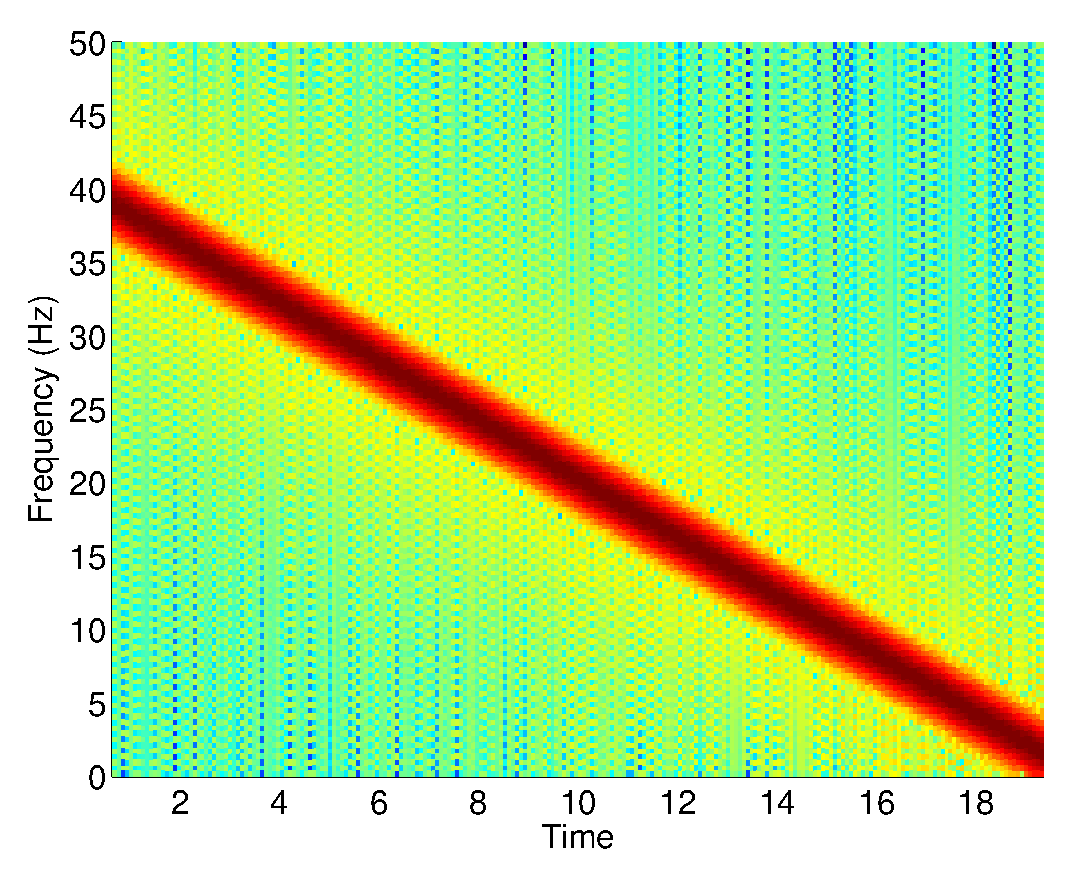
\includegraphics[width=4cm]{./Figures/Spect5.eps}
        \end{column}
      \end{columns}
      }
    \end{itemize}
  \end{itemize}
\end{frame}


\end{document}
